\documentclass[xcolor=dvipsnames]{beamer}

\newcommand{\set}[1]{\left\{ #1 \right\}}
\newcommand{\abs}[1]{\left\lvert #1 \right\rvert}

\newcommand{\N}{\mathbb{N}}
\newcommand{\Z}{\mathbb{Z}}
\newcommand{\R}{\mathbb{R}}
\newcommand{\F}{\mathbb{F}}
\renewcommand{\S}{\mathfrak{S}}

\newcommand{\Top}{\mathsf{Top}}
\newcommand{\Grp}{\mathsf{Grp}}
\newcommand{\Ab}{\mathsf{Ab}}
\newcommand{\Simp}{\mathsf{Simp}}
\newcommand{\Ch}{\mathsf{Ch}}


\makeatletter
\newcommand*{\defeq}{\mathrel{\rlap{%
    \raisebox{0.3ex}{$\m@th\cdot$}}%
  \raisebox{-0.3ex}{$\m@th\cdot$}}%
	=
}
\makeatother

\DeclareMathOperator{\im}{im}

% Category theory
\newcommand{\longto}{\longrightarrow}
\newcommand{\into}{\hookrightarrow}

\newcommand{\MKNN}{M\( k \)NN }
\newcommand{\hombound}[2]{\bar{\partial}_{#1}^{#2}}
\newcommand{\hbound}[1]{\bar{\partial}^{#1}}

% Cycles and boundaries
\newcommand{\cyc}[1]{\ker{\partial}_{#1}}
\newcommand{\bound}[1]{\im{\partial}_{#1}}

\newcommand{\pcyc}[2]{\ker{\partial}_{#1}^{#2}}
\newcommand{\pbound}[2]{\im{\partial}_{#1}^{#2}}


\usepackage[english]{babel}
\usepackage[utf8]{inputenc}
\usepackage[T1]{fontenc}
\usepackage{lmodern}

\usepackage{graphicx}
\graphicspath{{figs/}{../figs/}}

\usepackage{amsmath, amssymb, mathtools}

\hypersetup{
	urlcolor = {red!50!blue},
	linktoc = page
}

\title[TDA and persistent homology]{\bfseries{Topological data analysis and persistent
homology}}
\subtitle{Developing an outlier detector based on persistent homology}
\author[Arnau Mas]{Arnau Mas}
\institute[]{\footnotesize{\itshape{Supervised by}} \\ Dr Albert Ruiz}
\date[UAB, Sept 9th 2020]{\small Universitat Autònoma de Barcelona \\ September 3rd 2020}
\titlegraphic{
\includegraphics[scale=0.1]{logo-uab}}

% Theme settings
\usetheme{Madrid}
\usecolortheme[named=MidnightBlue]{structure}
\useoutertheme[subsection=false]{miniframes}
\useinnertheme{circles}

% Move miniframes to footline
\setbeamertemplate{navigation symbols}{}
\setbeamertemplate{headline}{}
\setbeamertemplate{mini frame in other subsection}{}
\makeatletter
\setbeamertemplate{footline}
  {%
    \begin{beamercolorbox}[colsep=1.5pt]{lower separation line foot}
    \end{beamercolorbox}
      \begin{beamercolorbox}[colsep=1.5pt]{upper separation line head}
  \end{beamercolorbox}
  \begin{beamercolorbox}{section in head/foot}
    \vskip2pt\insertnavigation{\paperwidth}\vskip4pt
  \end{beamercolorbox}%
  \begin{beamercolorbox}[colsep=1.5pt]{lower separation line head}
  \end{beamercolorbox}
  }
\makeatother

% Add logo to title
\setbeamerfont{frametitle}{series=\bfseries}
\setbeamertemplate{frametitle}{%
  \nointerlineskip
    \begin{beamercolorbox}[sep=0.5ex,wd=\paperwidth,leftskip=.2cm,rightskip=0cm]{frametitle}%
      \usebeamerfont{frametitle}\usebeamercolor[fg]{frametitle}\insertframetitle
      \hfill
      \raisebox{-0.3\height}{
\includegraphics[scale = 0.04]{logo-uab-blanc}}
    \end{beamercolorbox}%
}

\begin{document}
\begin{frame}[plain]
	\titlepage
\end{frame}

\AtBeginSection[]{
\begin{frame}
	\frametitle{Outline}
	\tableofcontents[currentsection]
\end{frame}
}

\AtEndDocument{
	\begin{frame}[plain]
		\titlepage
	\end{frame}
}

\begin{frame}
	\frametitle{Outline}
	\tableofcontents
\end{frame}

\section{The problem}

\begin{frame}
	\frametitle{What is radiomics?}
	\begin{itemize}
		\item Has its origins in the field of oncology: tumour imaging \pause
		\item Extract many \alert{radiomic features} from scans \pause
		\item Look for correlations between radiomic features and treatment response
	\end{itemize}
\end{frame}

\begin{frame}
	\frametitle{What is radiomics?}
	\begin{columns}
		\begin{column}{0.4\textwidth}
			\begin{block}{Benefits}
				\begin{itemize}
					\item Non-invasive
					\item More systematic
					\item Quantitative
				\end{itemize} \pause
			\end{block}		
		\end{column}
		
		\begin{column}{0.4\textwidth}
			\begin{block}{Drawbacks}
				\begin{itemize}
					\item May be hard to reproduce
					\item High dimensional feature spaces
					\item Limited number of cases
				\end{itemize} 
			\end{block}				
		\end{column}
	\end{columns}
\end{frame}

\begin{frame}
	\frametitle{TOPiomics}

	\begin{center}
		
\includegraphics[width = 3cm]{beamer/logo-cvc}
		\quad
		
\includegraphics[width = 3cm]{beamer/logo-vhio}
	\end{center}

	\begin{itemize}
		\item TOPiomics is an ongoing collaboration between the Computer Vision Center (CVC) and the
			Vall d'Hebron Institute of Oncology (VHIO). \pause

		\item Main aim: early detection of patients with strange radiomic signatures,
			\emph{outliers}, for whom standard treatments could fail. \pause

		\item	Use \emph{topological data analysis}, hence TOPiomics (topological radiomics).

	\end{itemize}
\end{frame}

\begin{frame}
	\frametitle{Prior work}
	\begin{itemize}
		\item Progress thus far: use the \emph{mutual \( k \)-nearest neighbours} (\MKNN) graph to
			detect outliers. \pause
		\item Problem: there is a parameter that has to be fixed. It has to do with the scale
			at which we look at the data. \pause
		\item Idea: look at \emph{every} parameter value. \pause 
	\end{itemize}
	\centering \alert{This is persistence} 
\end{frame}

\section{An overview of homology}
\begin{frame}
	\frametitle{The elevator pitch}
	Algebraic topology studies topological spaces by computing algebraic invariants, namely
	with functors
	\begin{gather*}
		\Top \to \Grp \\ 
		\Top \to \Ab \\
		\Top \to \Ring \\
		\Top \to \Vect_K \\
				 \vdots
	\end{gather*}
	\pause
	Homology groups are one of these functors,
	\begin{equation*}
		H_n \colon \Top \to \Ab. 
	\end{equation*}
	\pause
	They come in many flavours, the simplest one is \emph{simplicial homology}, which works
	for \emph{simplicial complexes}. 
\end{frame}

\begin{frame}
	\frametitle{The ingredients of homology}
	\begin{columns}
		\begin{column}{0.5\textwidth}
			\begin{itemize}
				\item<1-> \emph{Simplex}. The convex hull of \alt<3->{an (ordered)}{a} set of
					\only<2->{(geometrically independent)} points. 
				\item<4-> \emph{Simplicial complex}, \( K \). Topological space assembled out of
					simplices glued along their faces. 
				\item<5-> \emph{Chain groups}, \( C_n(K) \). Free abelian groups generated by the \( n
					\)-simplices of a complex. 
			\end{itemize}		
		\end{column}

		\begin{column}{0.5\textwidth}
			\begin{center}
				\only<1-3>{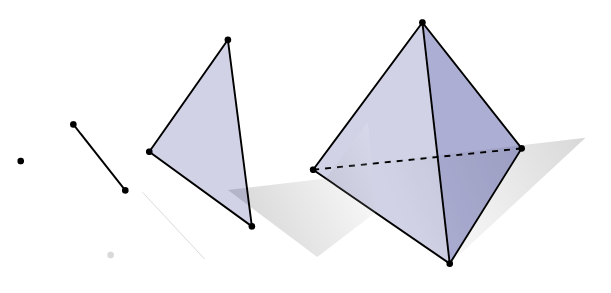
\includegraphics[scale=0.3]{beamer/simplices}}	
				\includegraphics<4->[scale=0.1]{beamer/complex}	
			\end{center}
		\end{column}
	\end{columns}
	
	\only<5>{
		\begin{block}{Remark}
			In the combinatorial picture, the geometrical requirements are dropped and one speaks
			of \emph{abstract} simplices, \emph{abstract} simplicial complexes, etc.
		\end{block}
	}

	\only<6>{
		\begin{block}{Remark}
			Free abelian groups are equivalent to \( \Z \)-modules. Alternatively, one can also
			consider the vector spaces generated by the chains, for instance over \( \F_2 \). 
		\end{block}
	}
\end{frame}

\begin{frame}
	\frametitle{The boundary morphism}
	\begin{block}{Orientation}
		The simplex generated by \( p_0, \dots, p_n \) is written \( [p_0, \dots, p_n] \). The
		ordering determines an orientation, and we require that flipping orientation implies a
		change of sign in \( C_n(K) \), e.g.
		\begin{equation*}
			[p_0, p_1, \dots, p_n] = -[p_1, p_0, \dots, p_n]. 
		\end{equation*}
		\pause
		The chain groups are not really free!
	\end{block}
\end{frame}

\begin{frame}
	\frametitle{The boundary morphisms}
	Define the boundary morphism \( \partial_n \colon C_n(K) \to C_{n-1}(K) \) by
	\begin{equation*}
		\partial_n [p_0, \dots, p_n] \defeq \sum_{k = 0}^{n} (-1)^k [p_0, \dots, \hat p_k,
		\dots, p_n]
	\end{equation*}
	and extending to chains. 
	\pause

	\centering{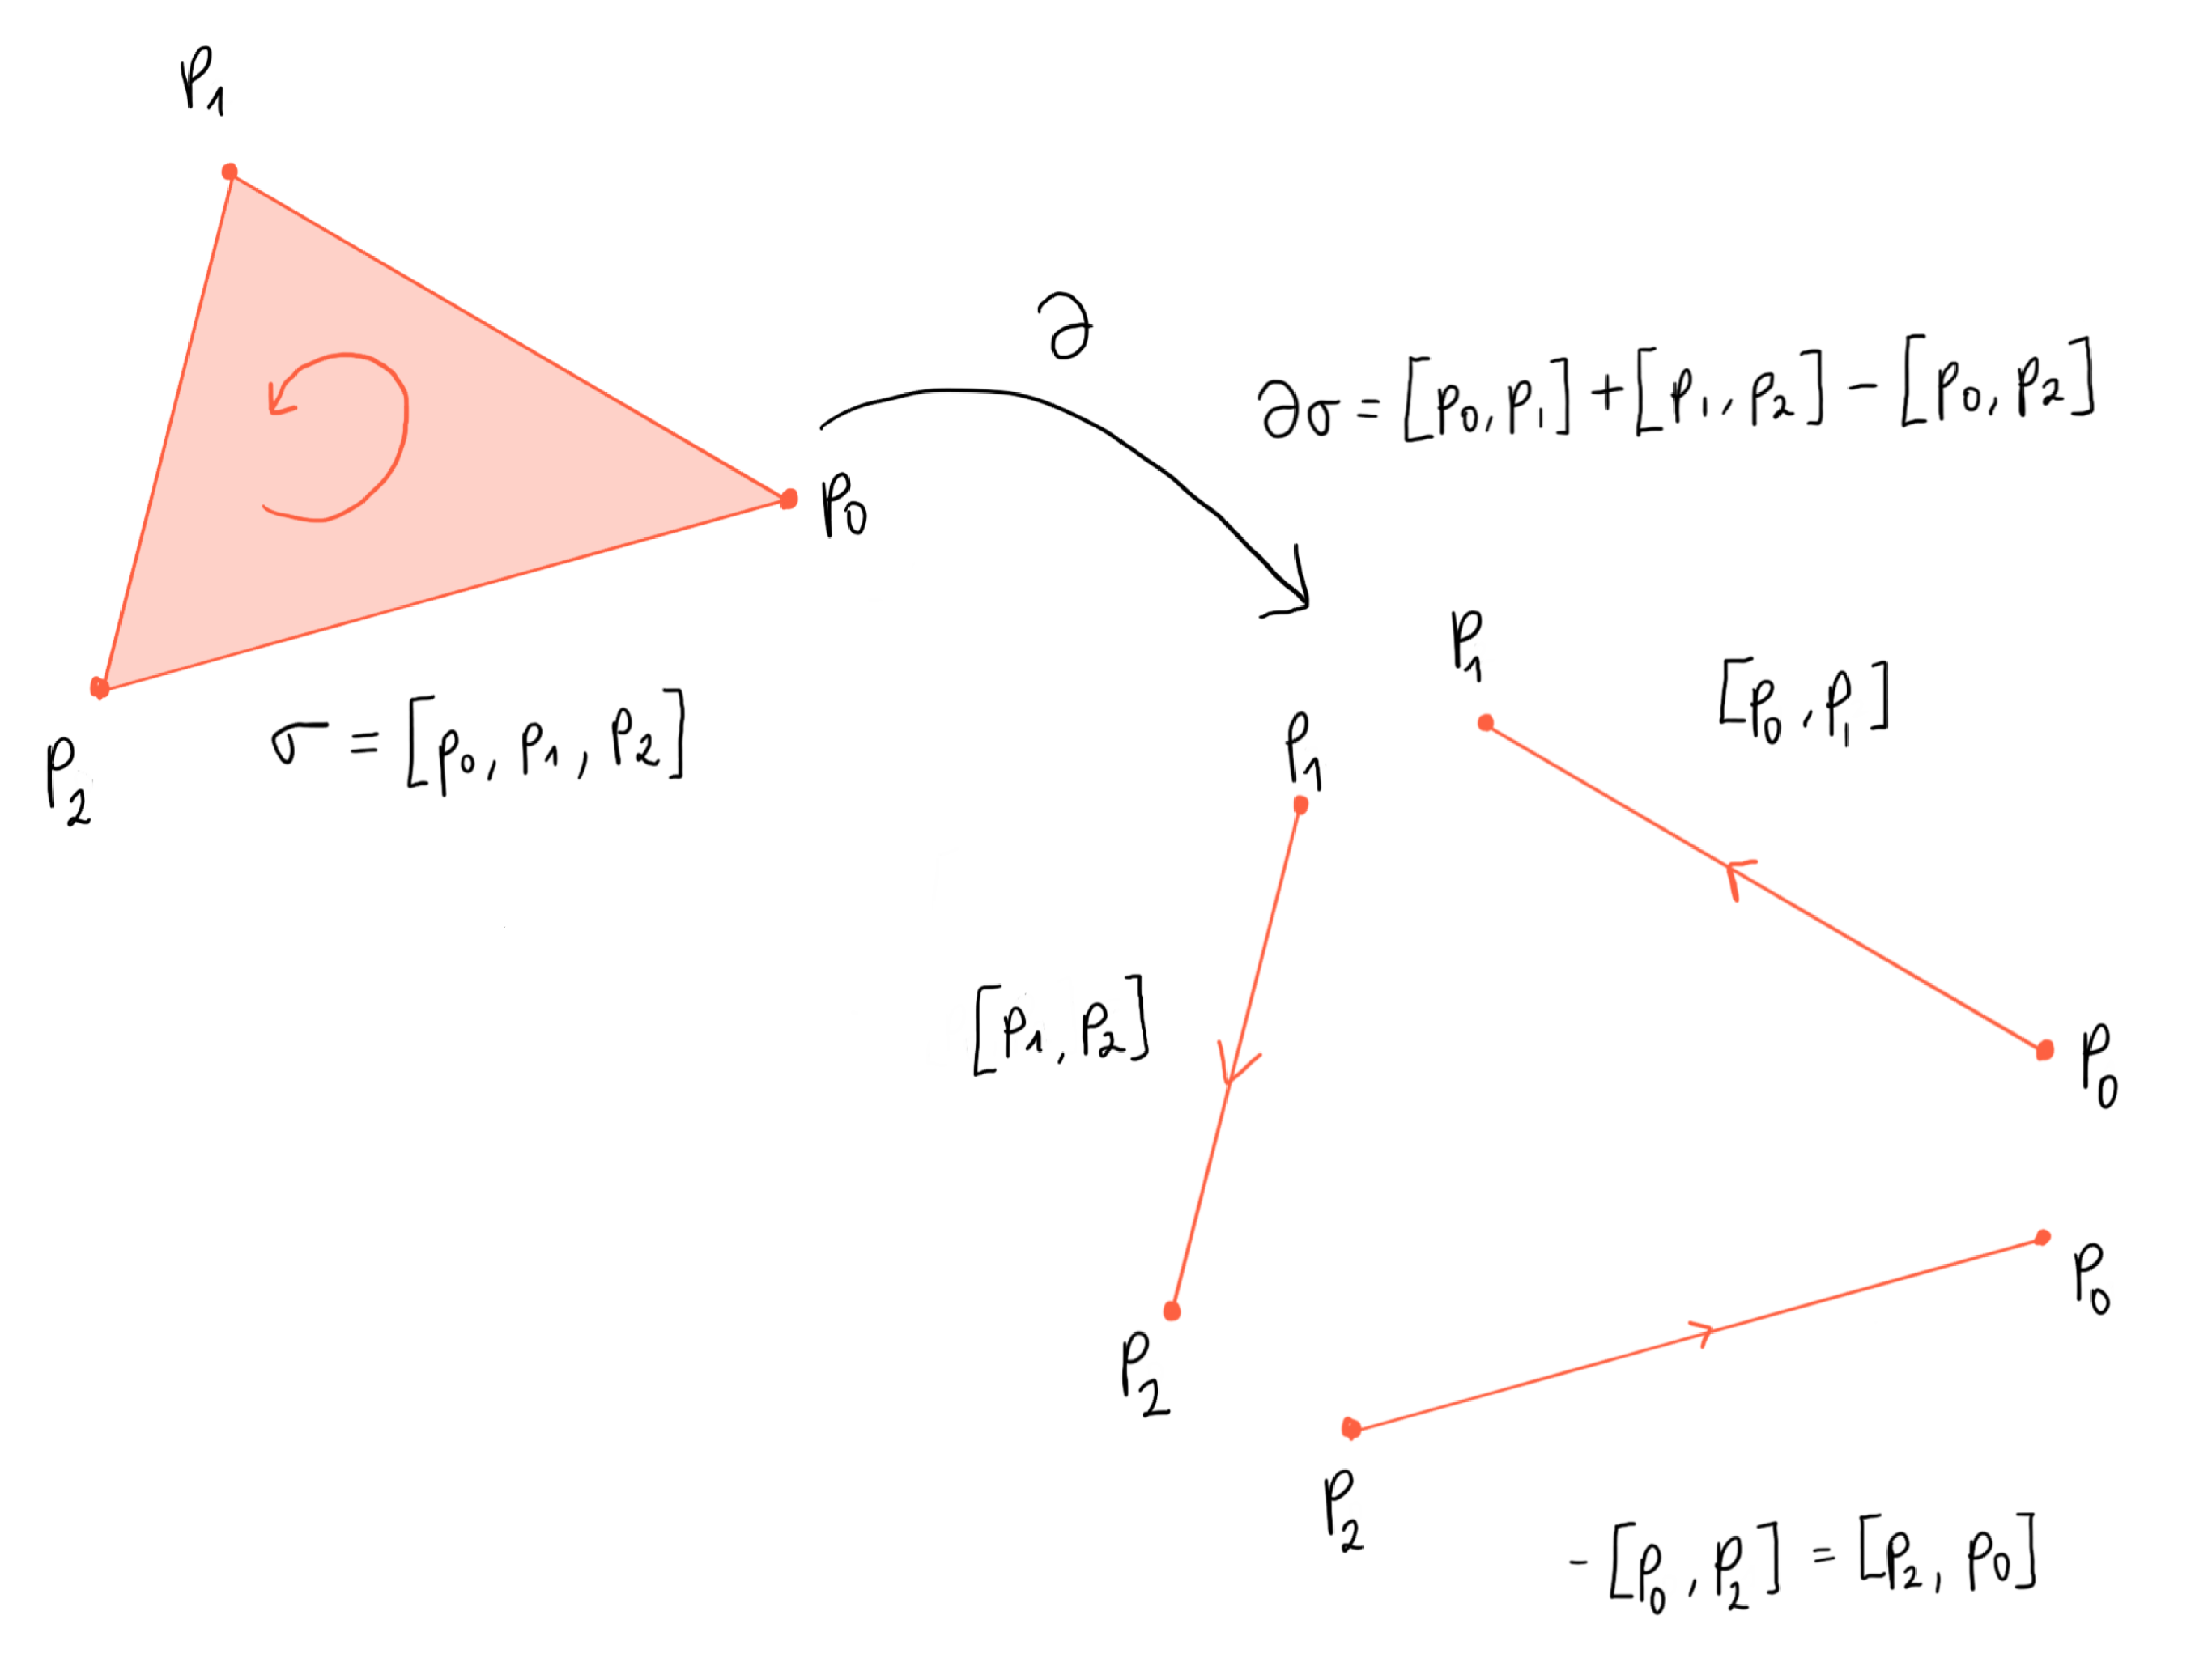
\includegraphics[width=0.6\textwidth]{drawings/boundary}}
\end{frame}	

\begin{frame}
	\frametitle{Boundaries and cycles}
	\begin{itemize}
		\item \emph{Cycles:} chains with no boundary,
			\begin{equation*}
				Z_n(K) \defeq \ker{\partial_n} \subseteq C_n(K)
			\end{equation*}
			\pause

		\item \emph{Boundaries:} chains which are the boundary of a higher-dimensional chain,
			\begin{equation*}
				B_n(K) \defeq \im{\partial_{n+1}} \subseteq C_n(K)
			\end{equation*}
		\pause

		\begin{block}{Fact}
			\begin{equation*}
				\partial_n \circ \partial_{n+1} = 0
			\end{equation*}
			so boundaries are always cycles. 
		\end{block}
			
	\end{itemize}
\end{frame}

\begin{frame}
	\frametitle{Homology groups}
	Homology groups are the quotients
	\begin{equation*}
		H_n(K) \defeq Z_n(K)/B_n(K).
	\end{equation*}
	\pause
	
	The key insight: Homology groups measure \alert{cycles which are not boundaries.} \pause
	They tell us about the number of \( n \)-dimensional holes in our space. 
	
	\pause
	Homology is invariant under homotopy, weaker than invariance under homeomorphism. 
	
	
\end{frame}

\begin{frame}
	\frametitle{What is persistence?}
	Instead of a single simplicial complex, consider a \emph{filtration},
	\begin{equation*}
		K^0 \subseteq K^1 \subseteq \cdots \subseteq K^N.
	\end{equation*}
	\pause
	Then look at this evolution at the level of homology
	\only<1>{
		\begin{equation*}
			H_d^0(K) \into H_d^1(K) \into \cdots \into H_d^N(K)
		\end{equation*}
	}
	\only<2>{
		\begin{equation*}
			H_{\textcolor{red}{d}}^0(K)
			\into H_{\textcolor{red}{d}}^1(K) 
			\into \cdots 
			\into H_{\textcolor{red}{d}}^N(K) 
		\end{equation*}
	}
	\only<3>{
		\begin{equation*}
			H_d^{\textcolor{red}{0}}(K)
			\into H_d^{\textcolor{red}{1}}(K) 
			\into \cdots 
			\into H_d^{\textcolor{red}{N}}(K) 
		\end{equation*}
	}

	\uncover<3>{The steps of the filtration can be thought of as time}
\end{frame}

\begin{frame}
	\frametitle{What is persistence?}
	Because of functoriality, there are maps between the different steps of homology,
	\begin{equation*}
		f_i^j \colon H_d^i(K) \to H_d^j(K).
	\end{equation*}
	\pause
	At each step, classes can be born (not in the image of \( f_i^{i+1} \)), die (in the
	kernel of \( f_i^{i+1} \)) or merge (have the same image through \( f_i^{i+1} \)).
\end{frame}

\begin{frame}
	\frametitle{An example}
	\centering
	\only<1>{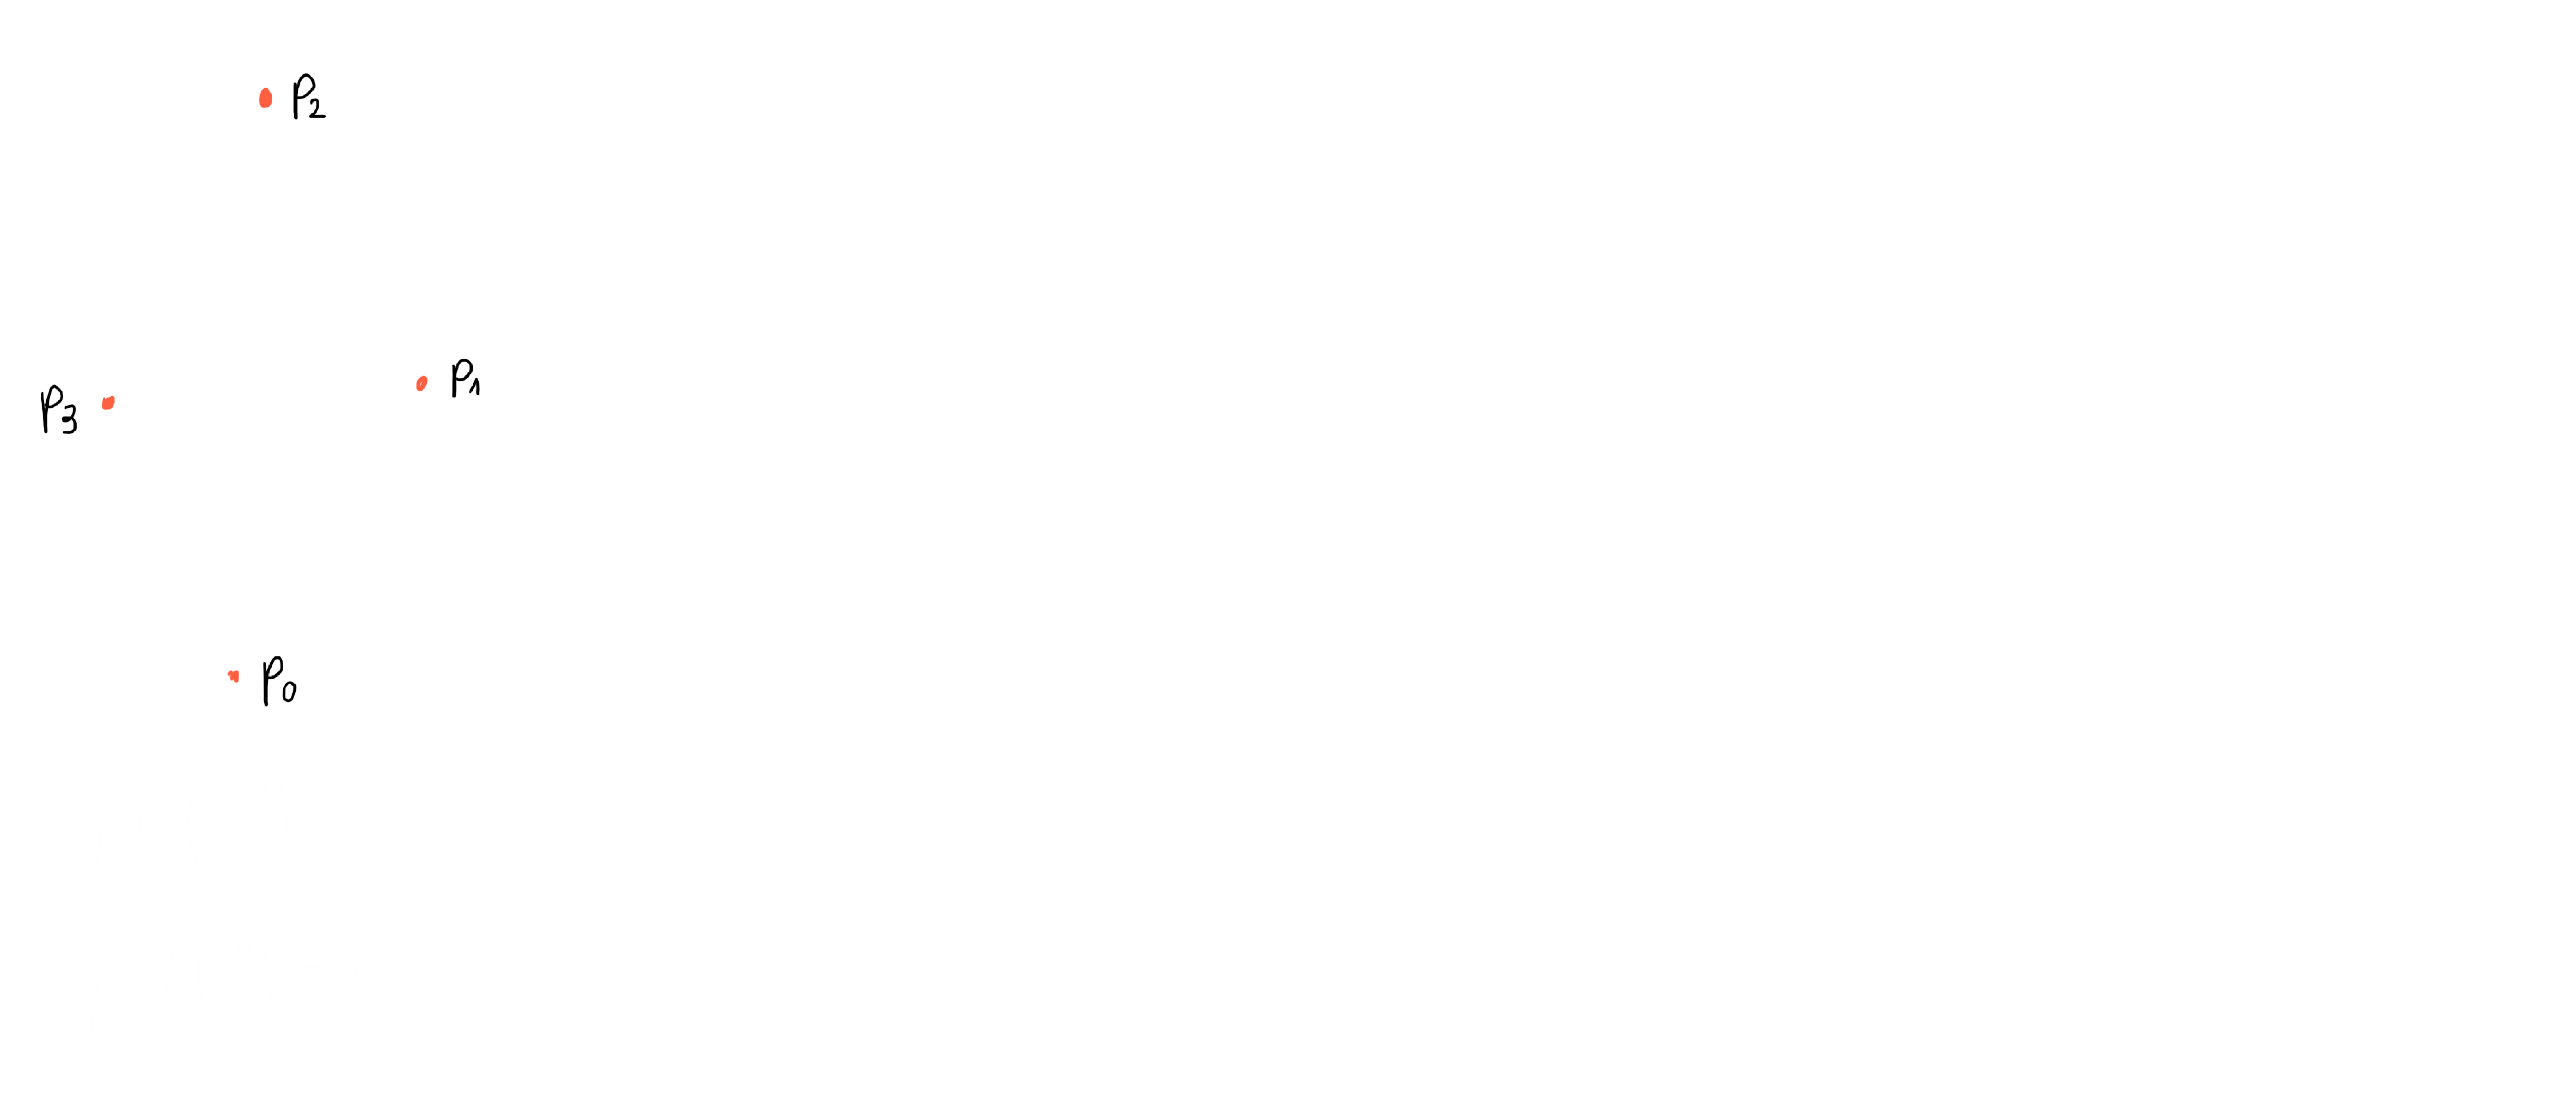
\includegraphics[width=\textwidth]{beamer/filt-1}}
	\only<2>{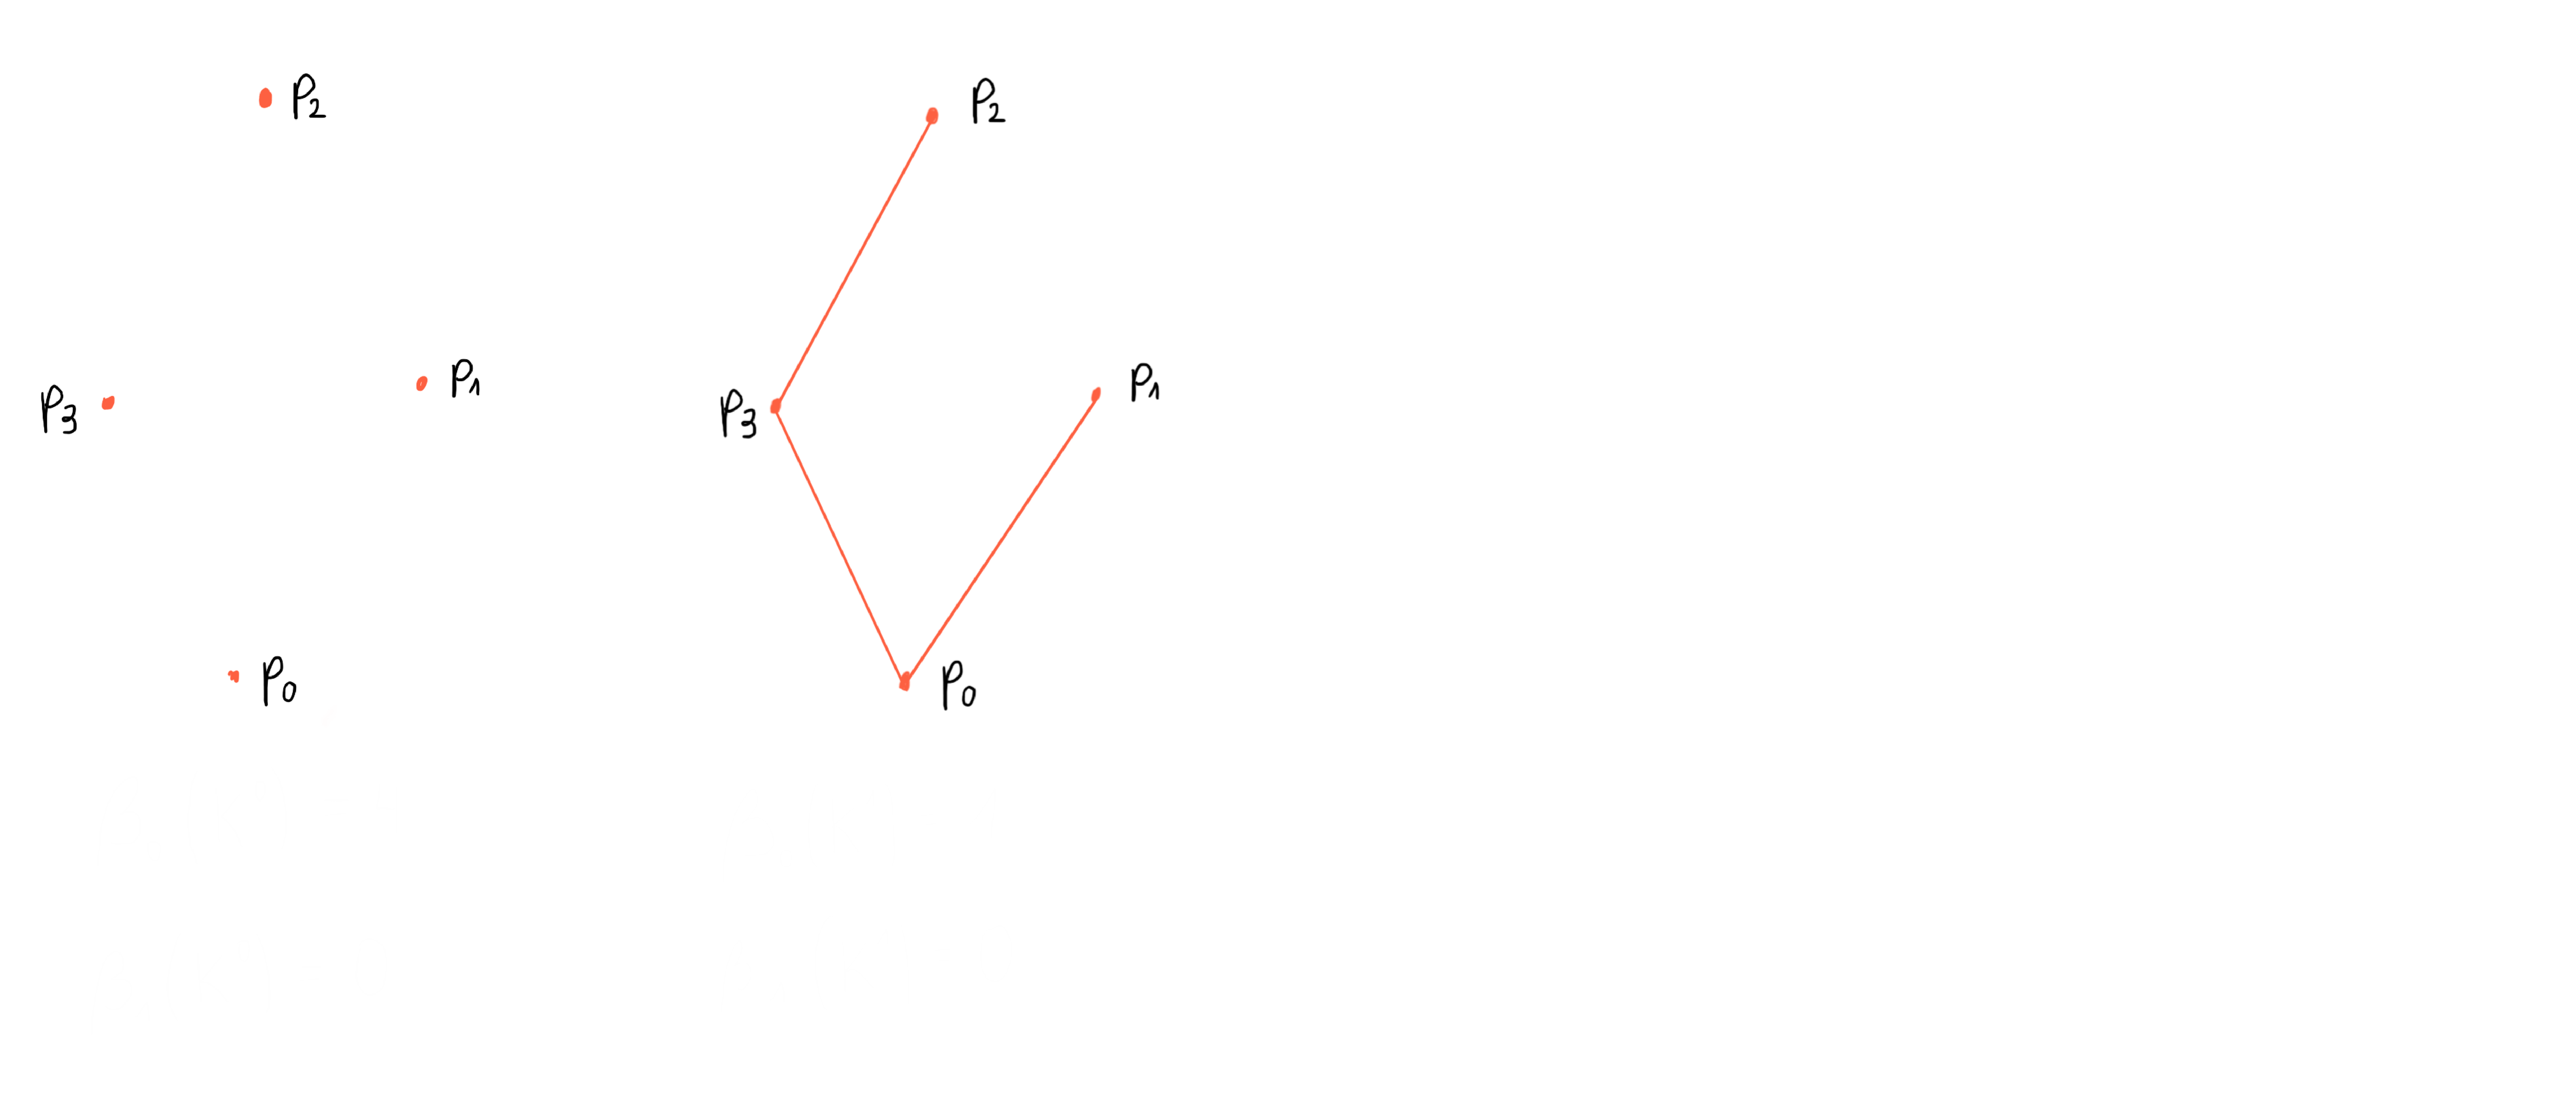
\includegraphics[width=\textwidth]{beamer/filt-2}}
	\only<3>{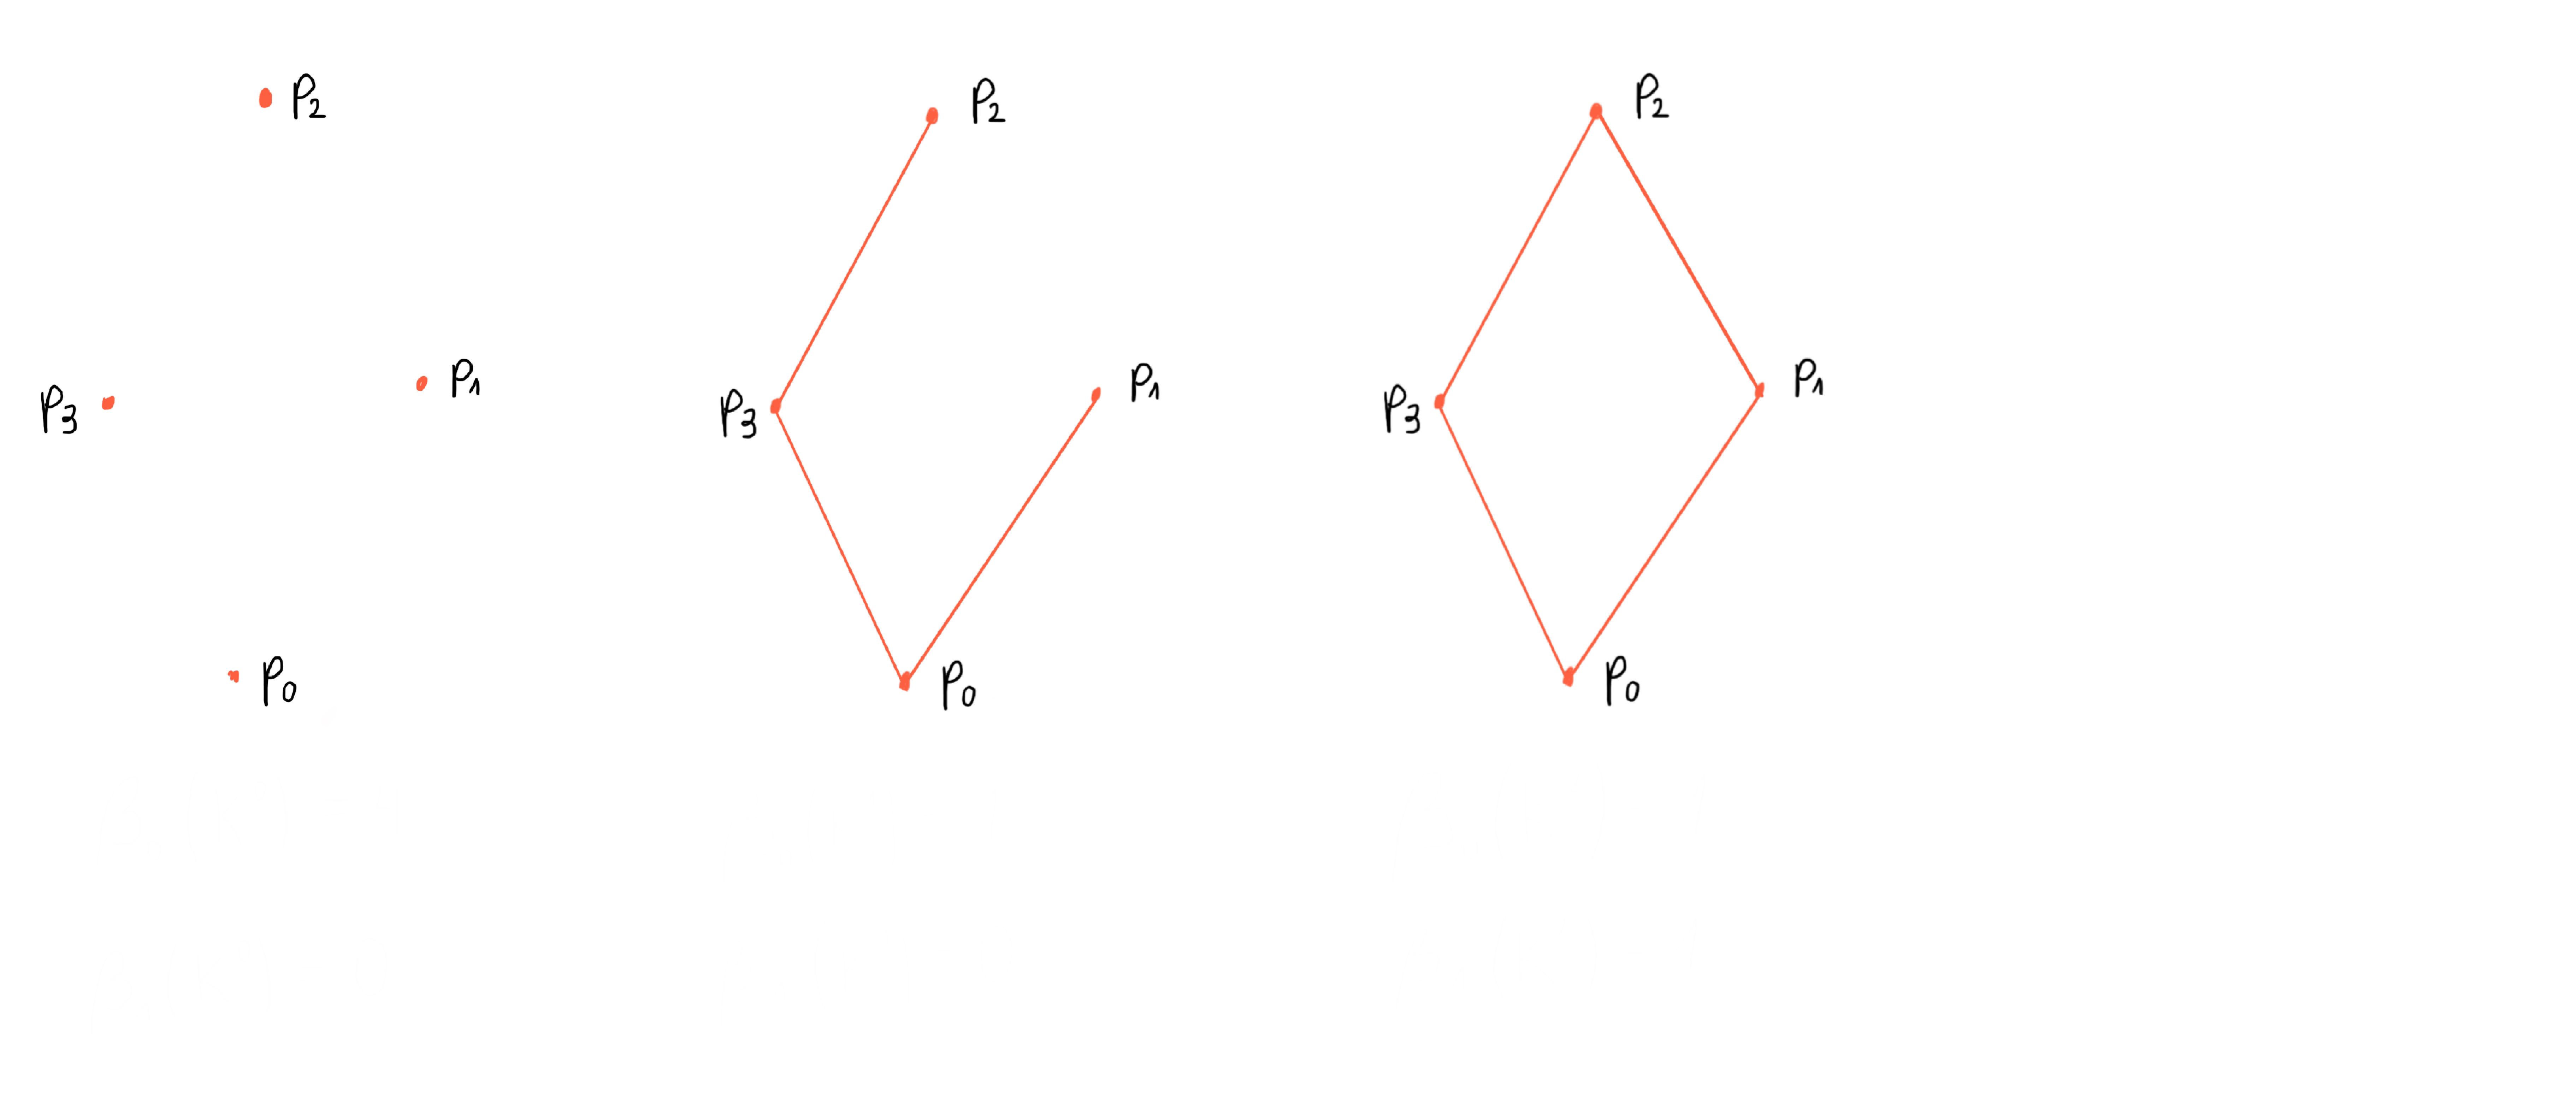
\includegraphics[width=\textwidth]{beamer/filt-3}}
	\only<4>{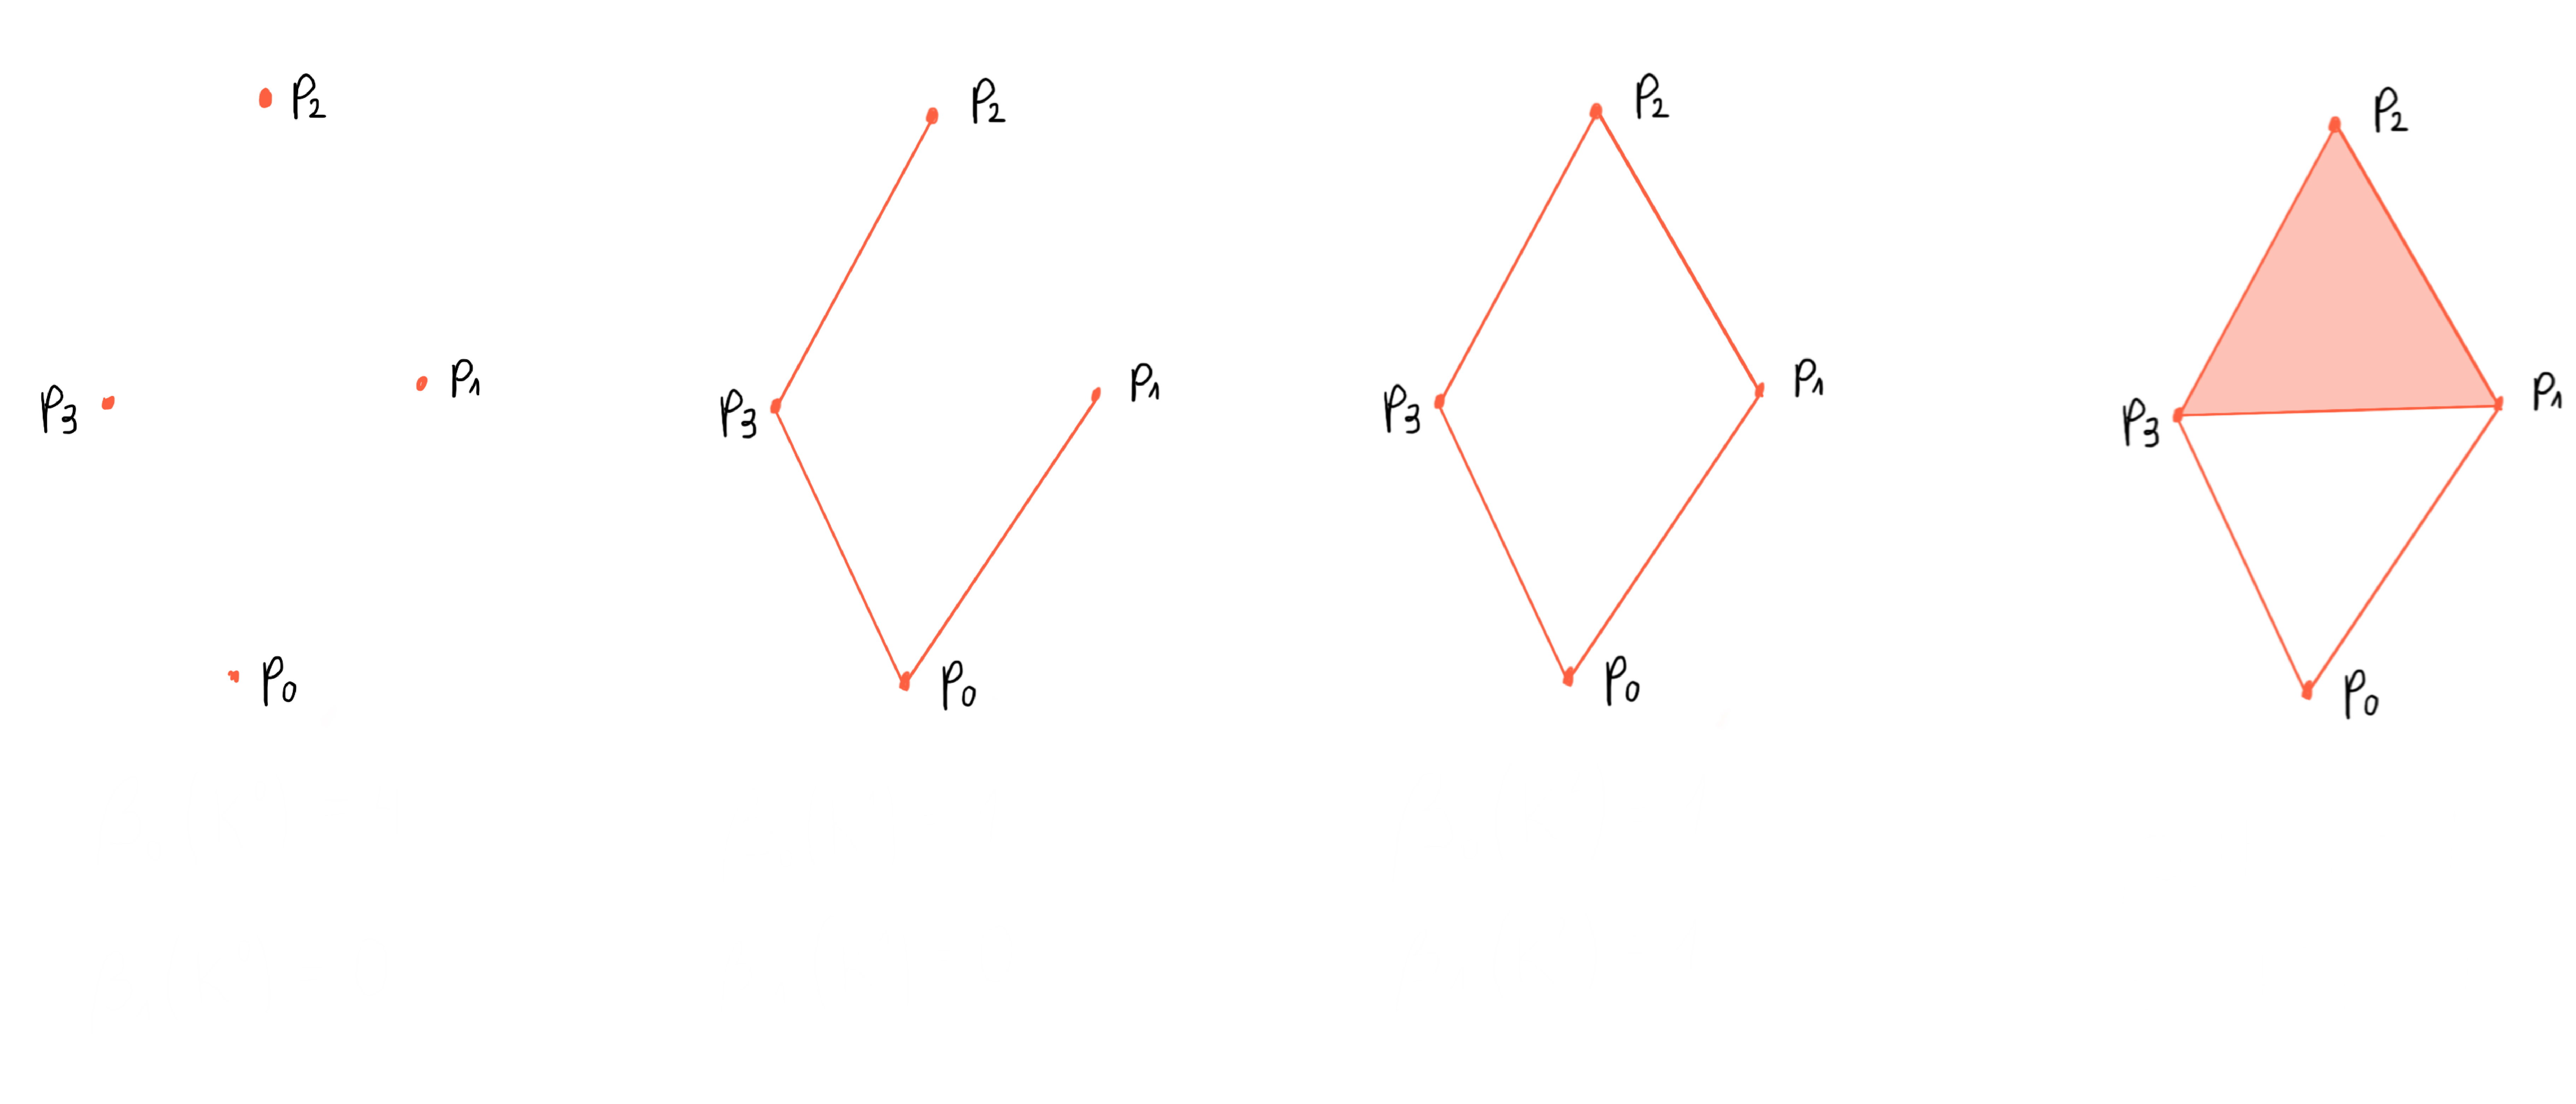
\includegraphics[width=\textwidth]{beamer/filt-4}}

	\only<1>{\( [p_0], [p_1], [p_2], [p_3] \) are born.}
	\only<2>{\( [p_0], [p_1], [p_2], [p_3] \) merge.}
	\only<3>{The cycle \( [p_0,p_1] + [p_1,p_2] + [p_2,p_3] + [p_3,p_4] \) is born.}
	\only<4>{The cycle does not die.}
\end{frame}

\section{The detector}
\begin{frame}
	\frametitle{Why the \MKNN graph?}
	It is good for detecting clusters in a data set. 
	\begin{center}
		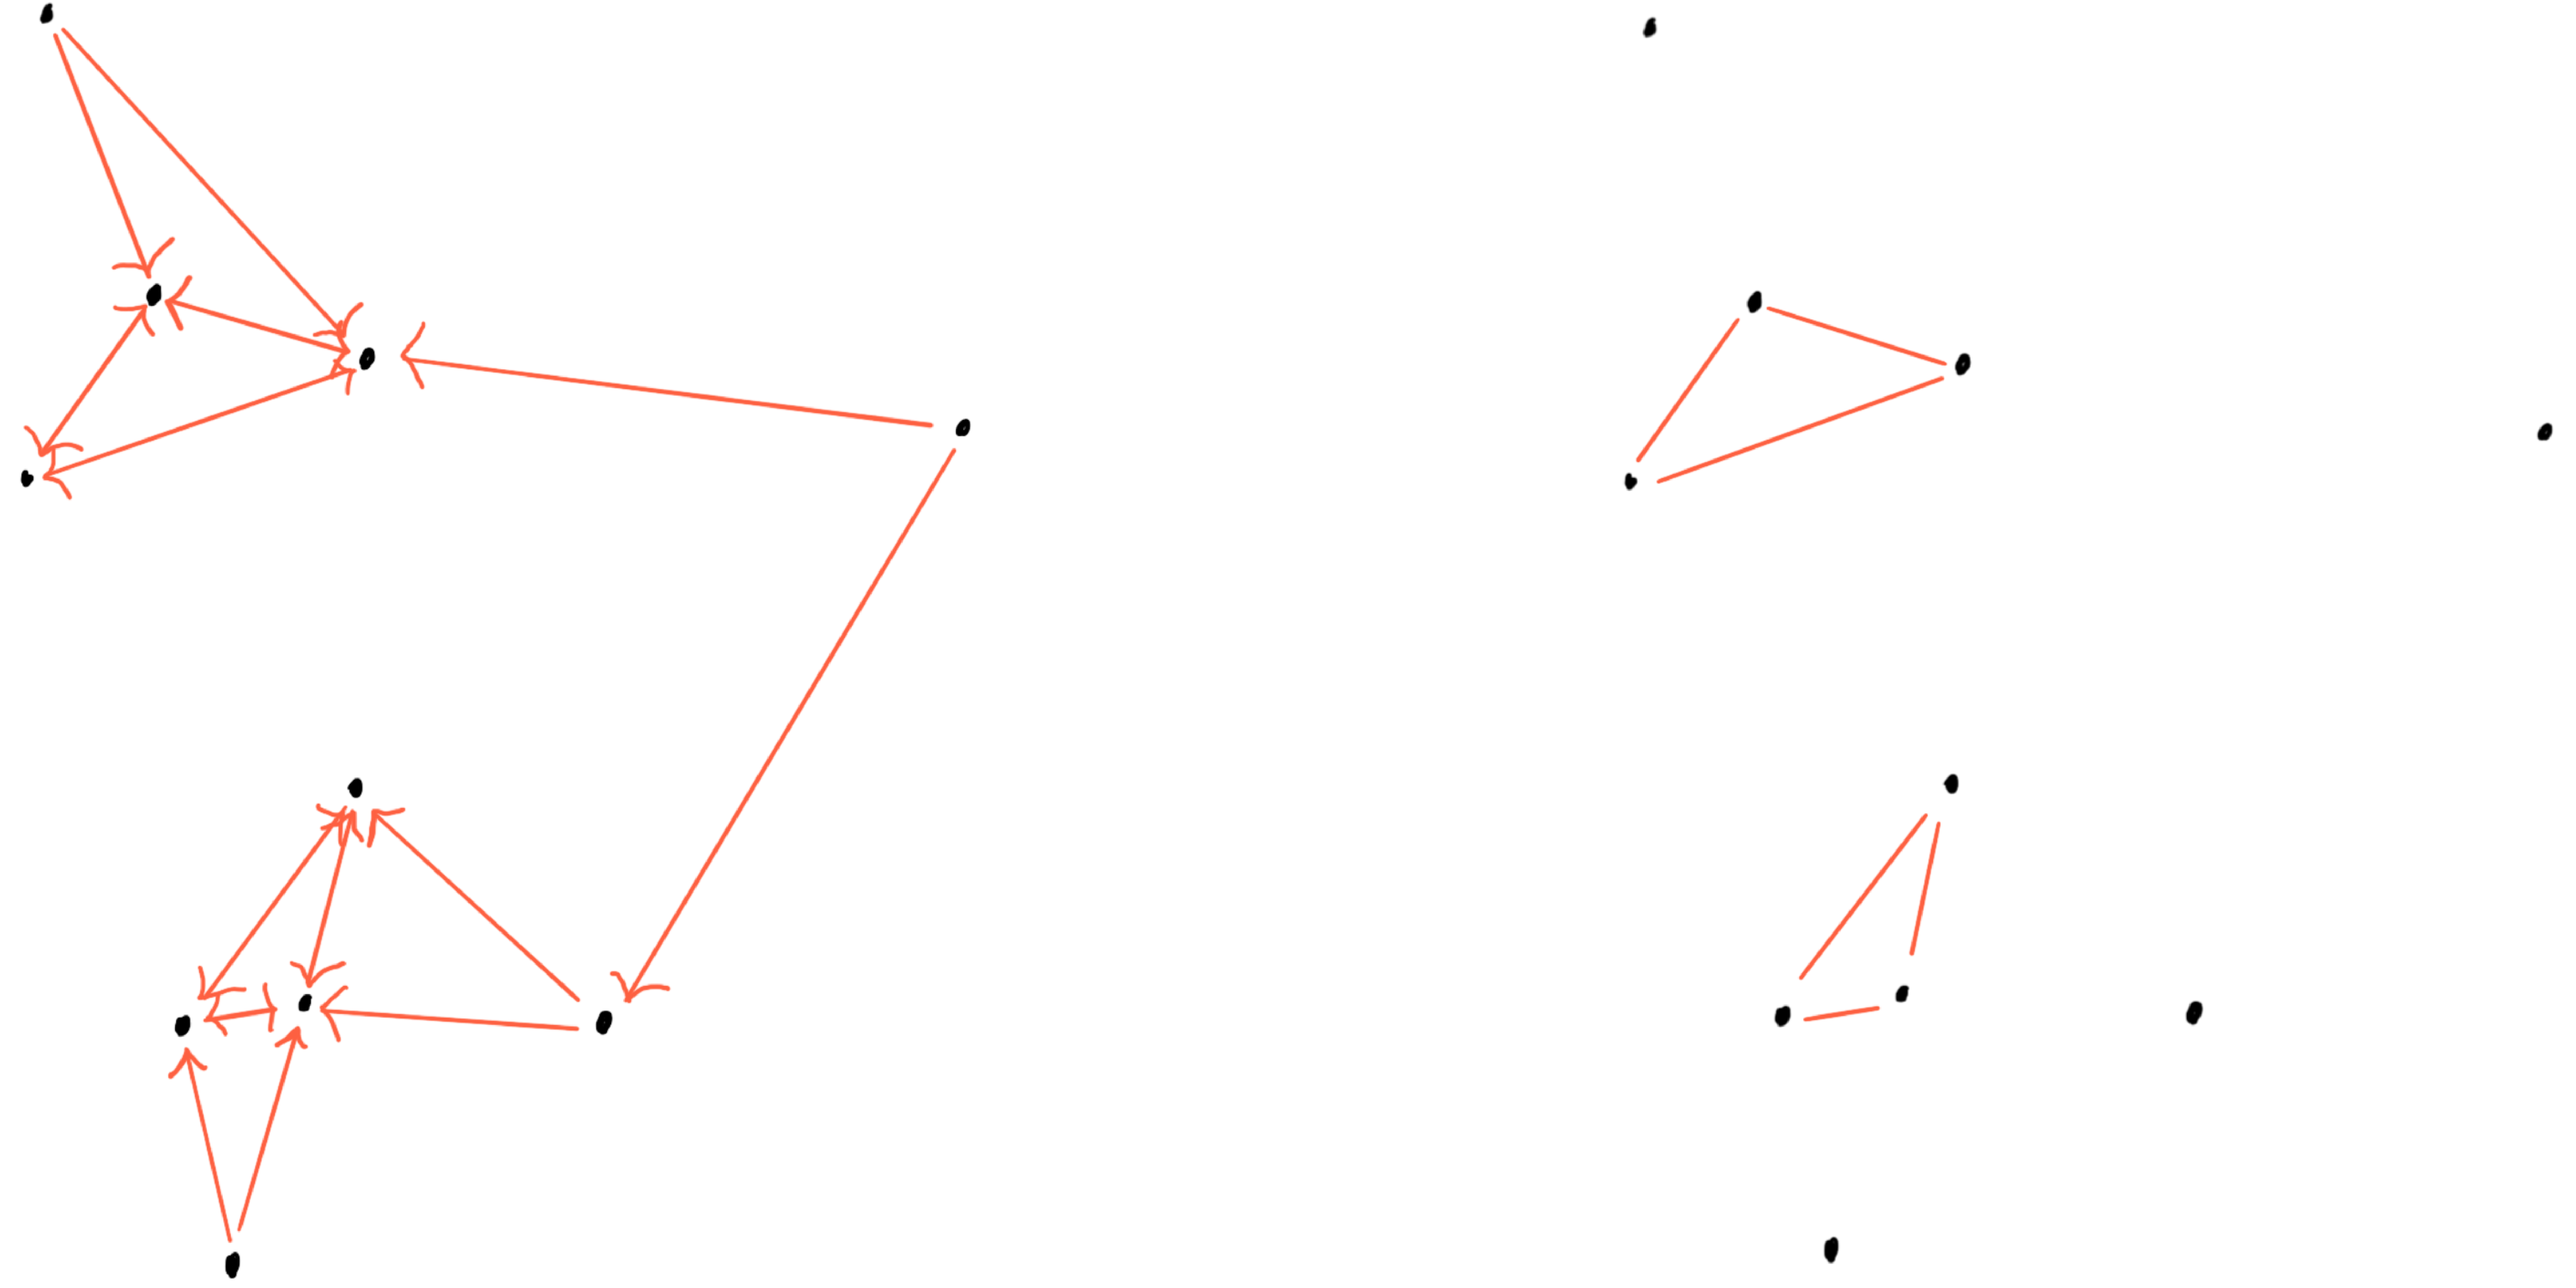
\includegraphics[width=\textwidth]{drawings/mknn}
	\end{center}
\end{frame}

\begin{frame}
	\frametitle{The outlier detection algorithm}
	The algorithm has four main parts: \pause
	\begin{itemize}
		\item The class \texttt{Cloud} stores a point cloud and computes its \MKNN graph.
			\pause
		\item The class \texttt{Filtration} builds up the filtration. \pause
		\item The class \texttt{Homology} computes the homology. \pause
		\item The persistence data of each class is gathered and plotted to detect the
			outliers. 
	\end{itemize}
	\pause
	All of the Python code is available at \url{github.com/arnaumas/mknn-homology}. 
\end{frame}

\begin{frame}
	\frametitle{The class \texttt{Cloud}}
	\begin{itemize}
		\item Store the cloud of \( N \) points in \( \R^d \) as a NumPy array of shape \(
			(N,d) \). \pause
		\item Construct the adjacency matrix, \( A \), of the \( k \)-nearest neighbours graph
			of the cloud. \pause
		\item The adjacency matrix of the the \MKNN graph is
			\begin{equation*}
				M = A \odot A^\top
			\end{equation*}
			where \( \odot \) is the entrywise product.
	\end{itemize}
\end{frame}

\begin{frame}
	\frametitle{The class \texttt{Filtration}}
	\begin{itemize}
		\item The package NetworkX can compute the cliques of a graph. These correspond to the
			simplices of the \emph{graph complex} associated to the \MKNN graph of the cloud.
			\pause
		\item The simplices are ordered by order of appearance and dimension, which ensures
			any simplex is always preceded by its faces. 
	\end{itemize}
\end{frame}

\begin{frame}
	\frametitle{The class \texttt{Homology}}
	\begin{itemize}
		\item The classes \texttt{Simplex} and \texttt{Chain} model elements of the chain
			groups and underpin the following computations. \pause
		\item The chain group is taken over \( \F_2 \), which corresponds to disregarding
			orientation and simplifies computation. \pause
		\item There is a Python dictionary which keeps track of the homology class of every
			clique. This is a memoised version of the projection \( \pi \colon C_n(K) \to
			C_n(K)/B_n(K) \). \pause
	\end{itemize}
\end{frame}

\begin{frame}
	\frametitle{The class \texttt{Homology}}
	\begin{itemize}
		\item Iterating through the filtration, for every simplex \( \sigma \), the homology
			class of the sum of its faces, \( w_0 + \dots + w_n \). \pause
			\item If it is zero, then before \( \sigma \) appears, there is chain \(
				c \) such that
				\begin{equation*}
					w_0 + \dots + w_n = \partial c.
				\end{equation*}
				\pause
				Once \( \sigma \) is added,
				\begin{equation*}
					w_0 + \cdots + w_n = \partial c = \partial \sigma
				\end{equation*}
			so \( \partial(\sigma + c) = 0 \), which means \( \sigma + c \) is a new cycle. 
	\end{itemize}
\end{frame}

\begin{frame}
	\frametitle{The class \texttt{Homology}}
	\centering
	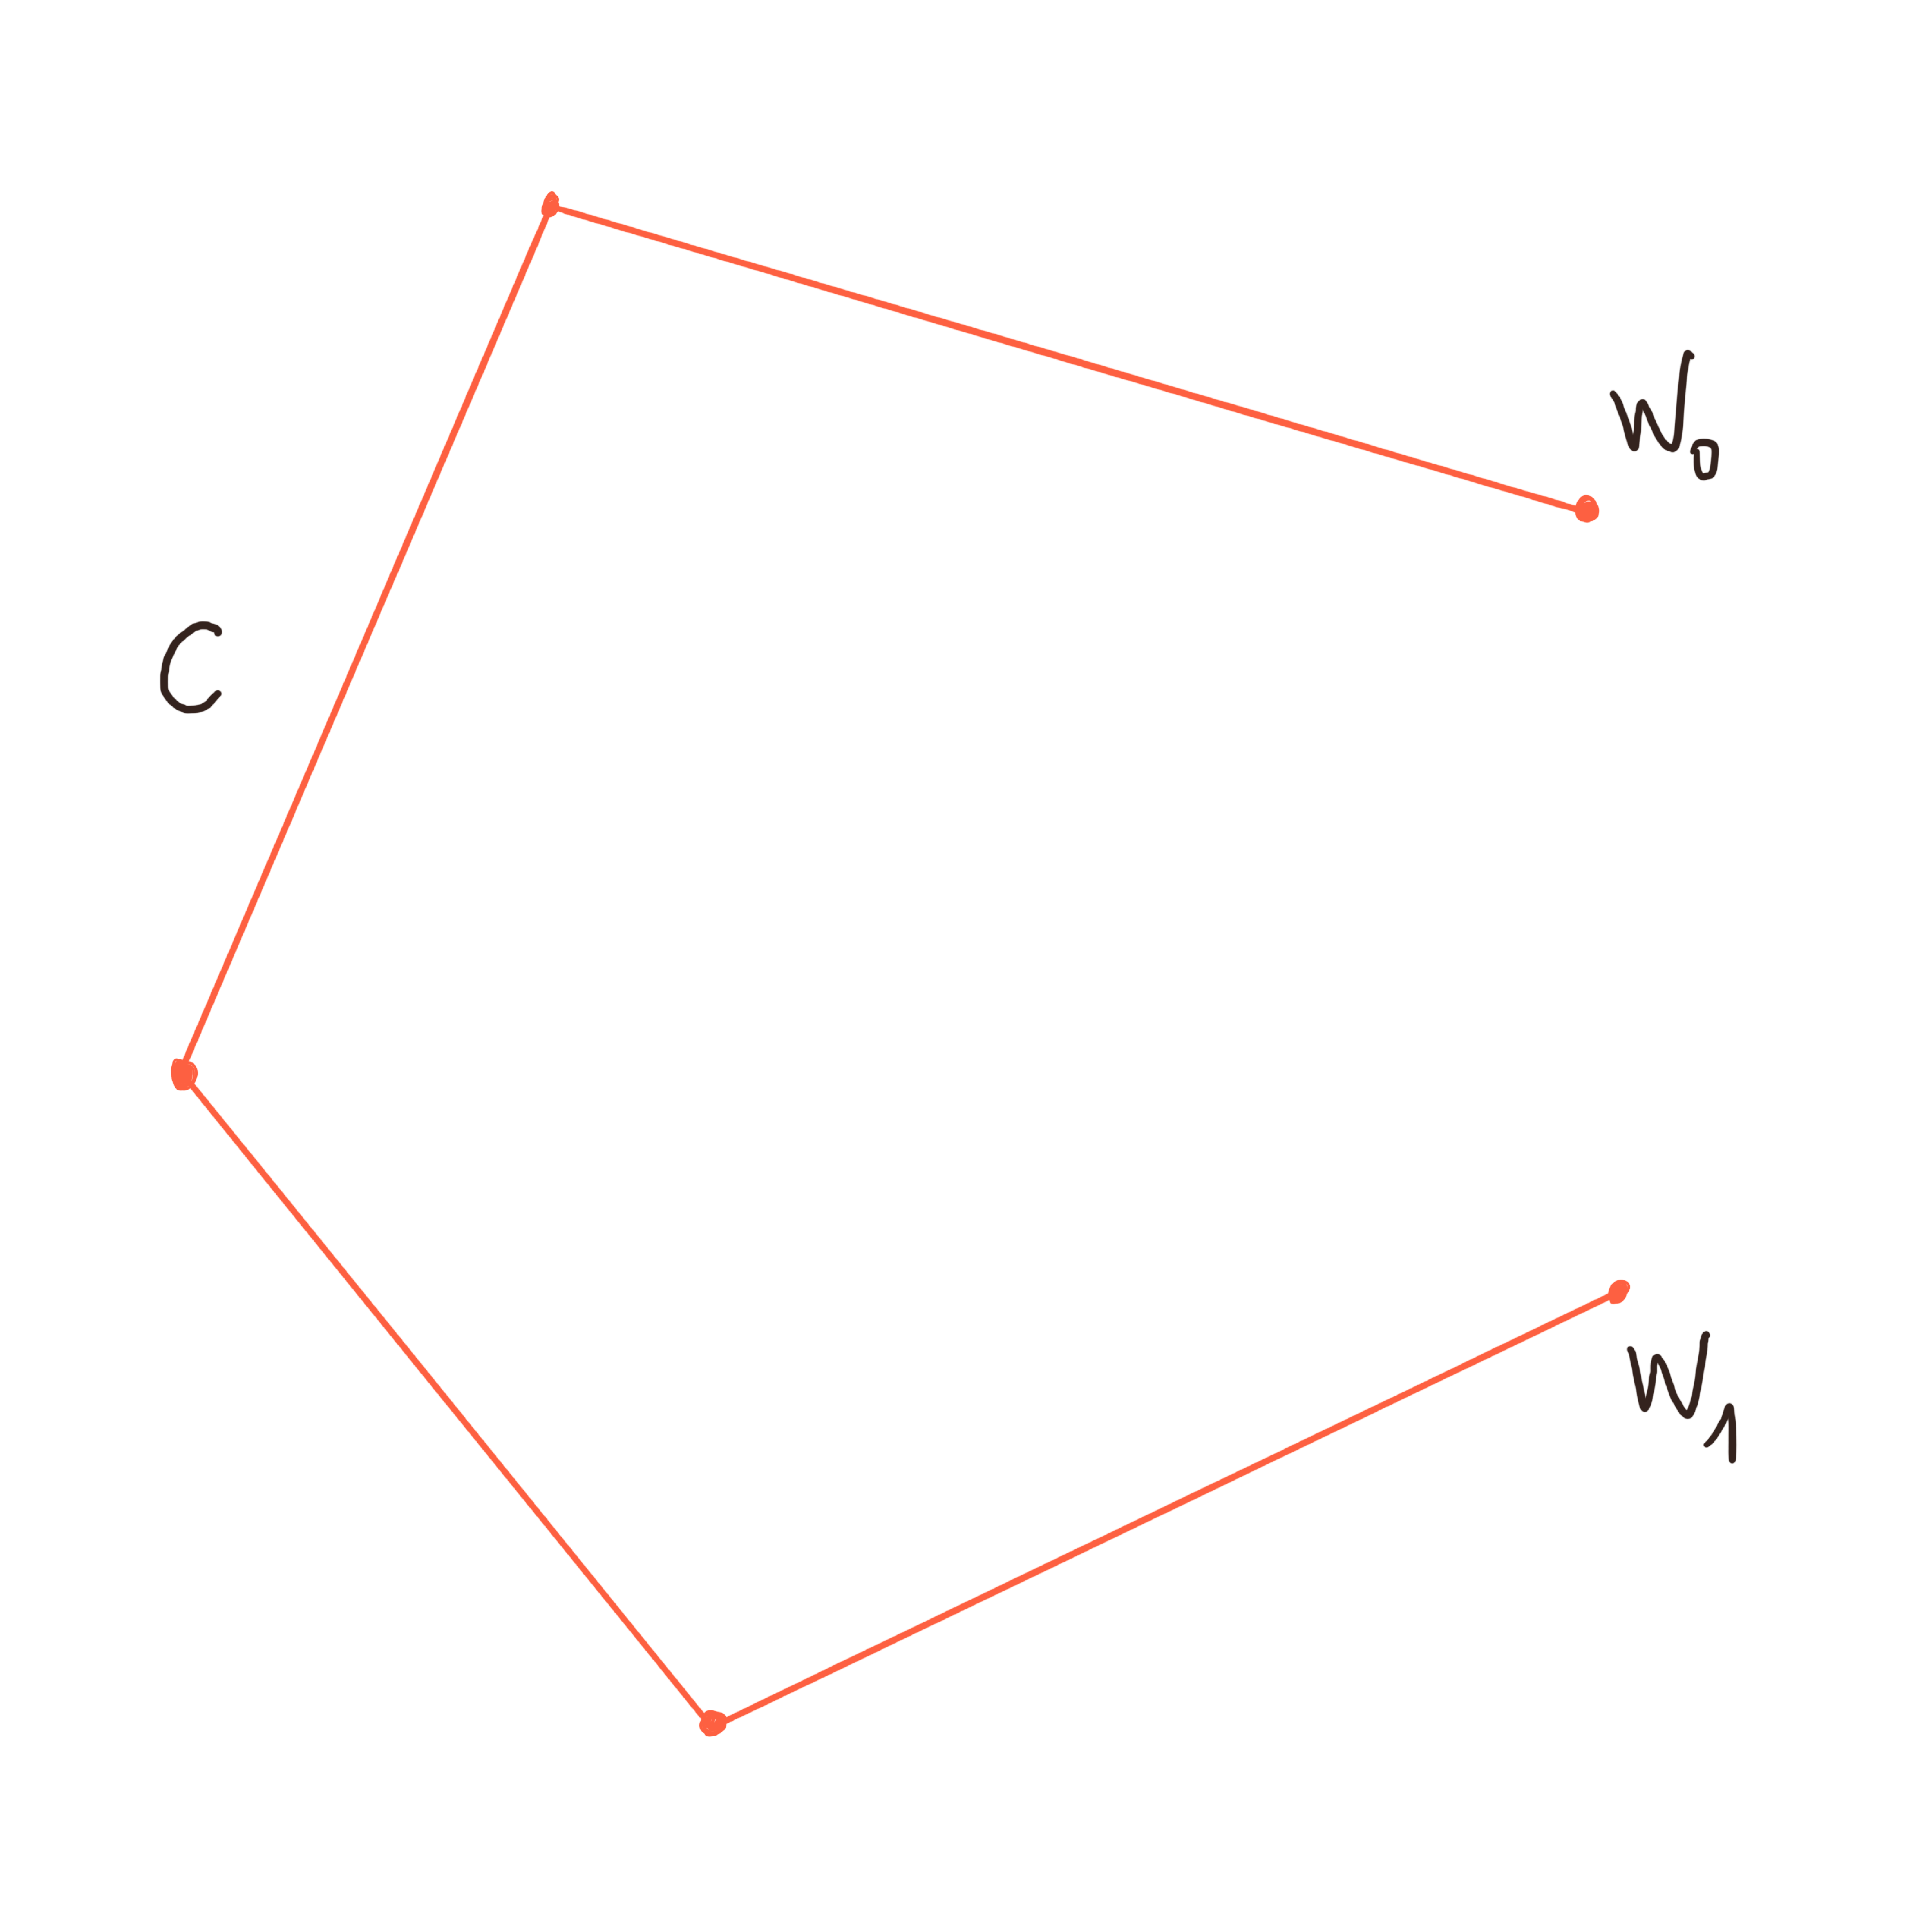
\includegraphics[width = 0.4\textwidth]{beamer/close-1}
	\hfill
	\pause
	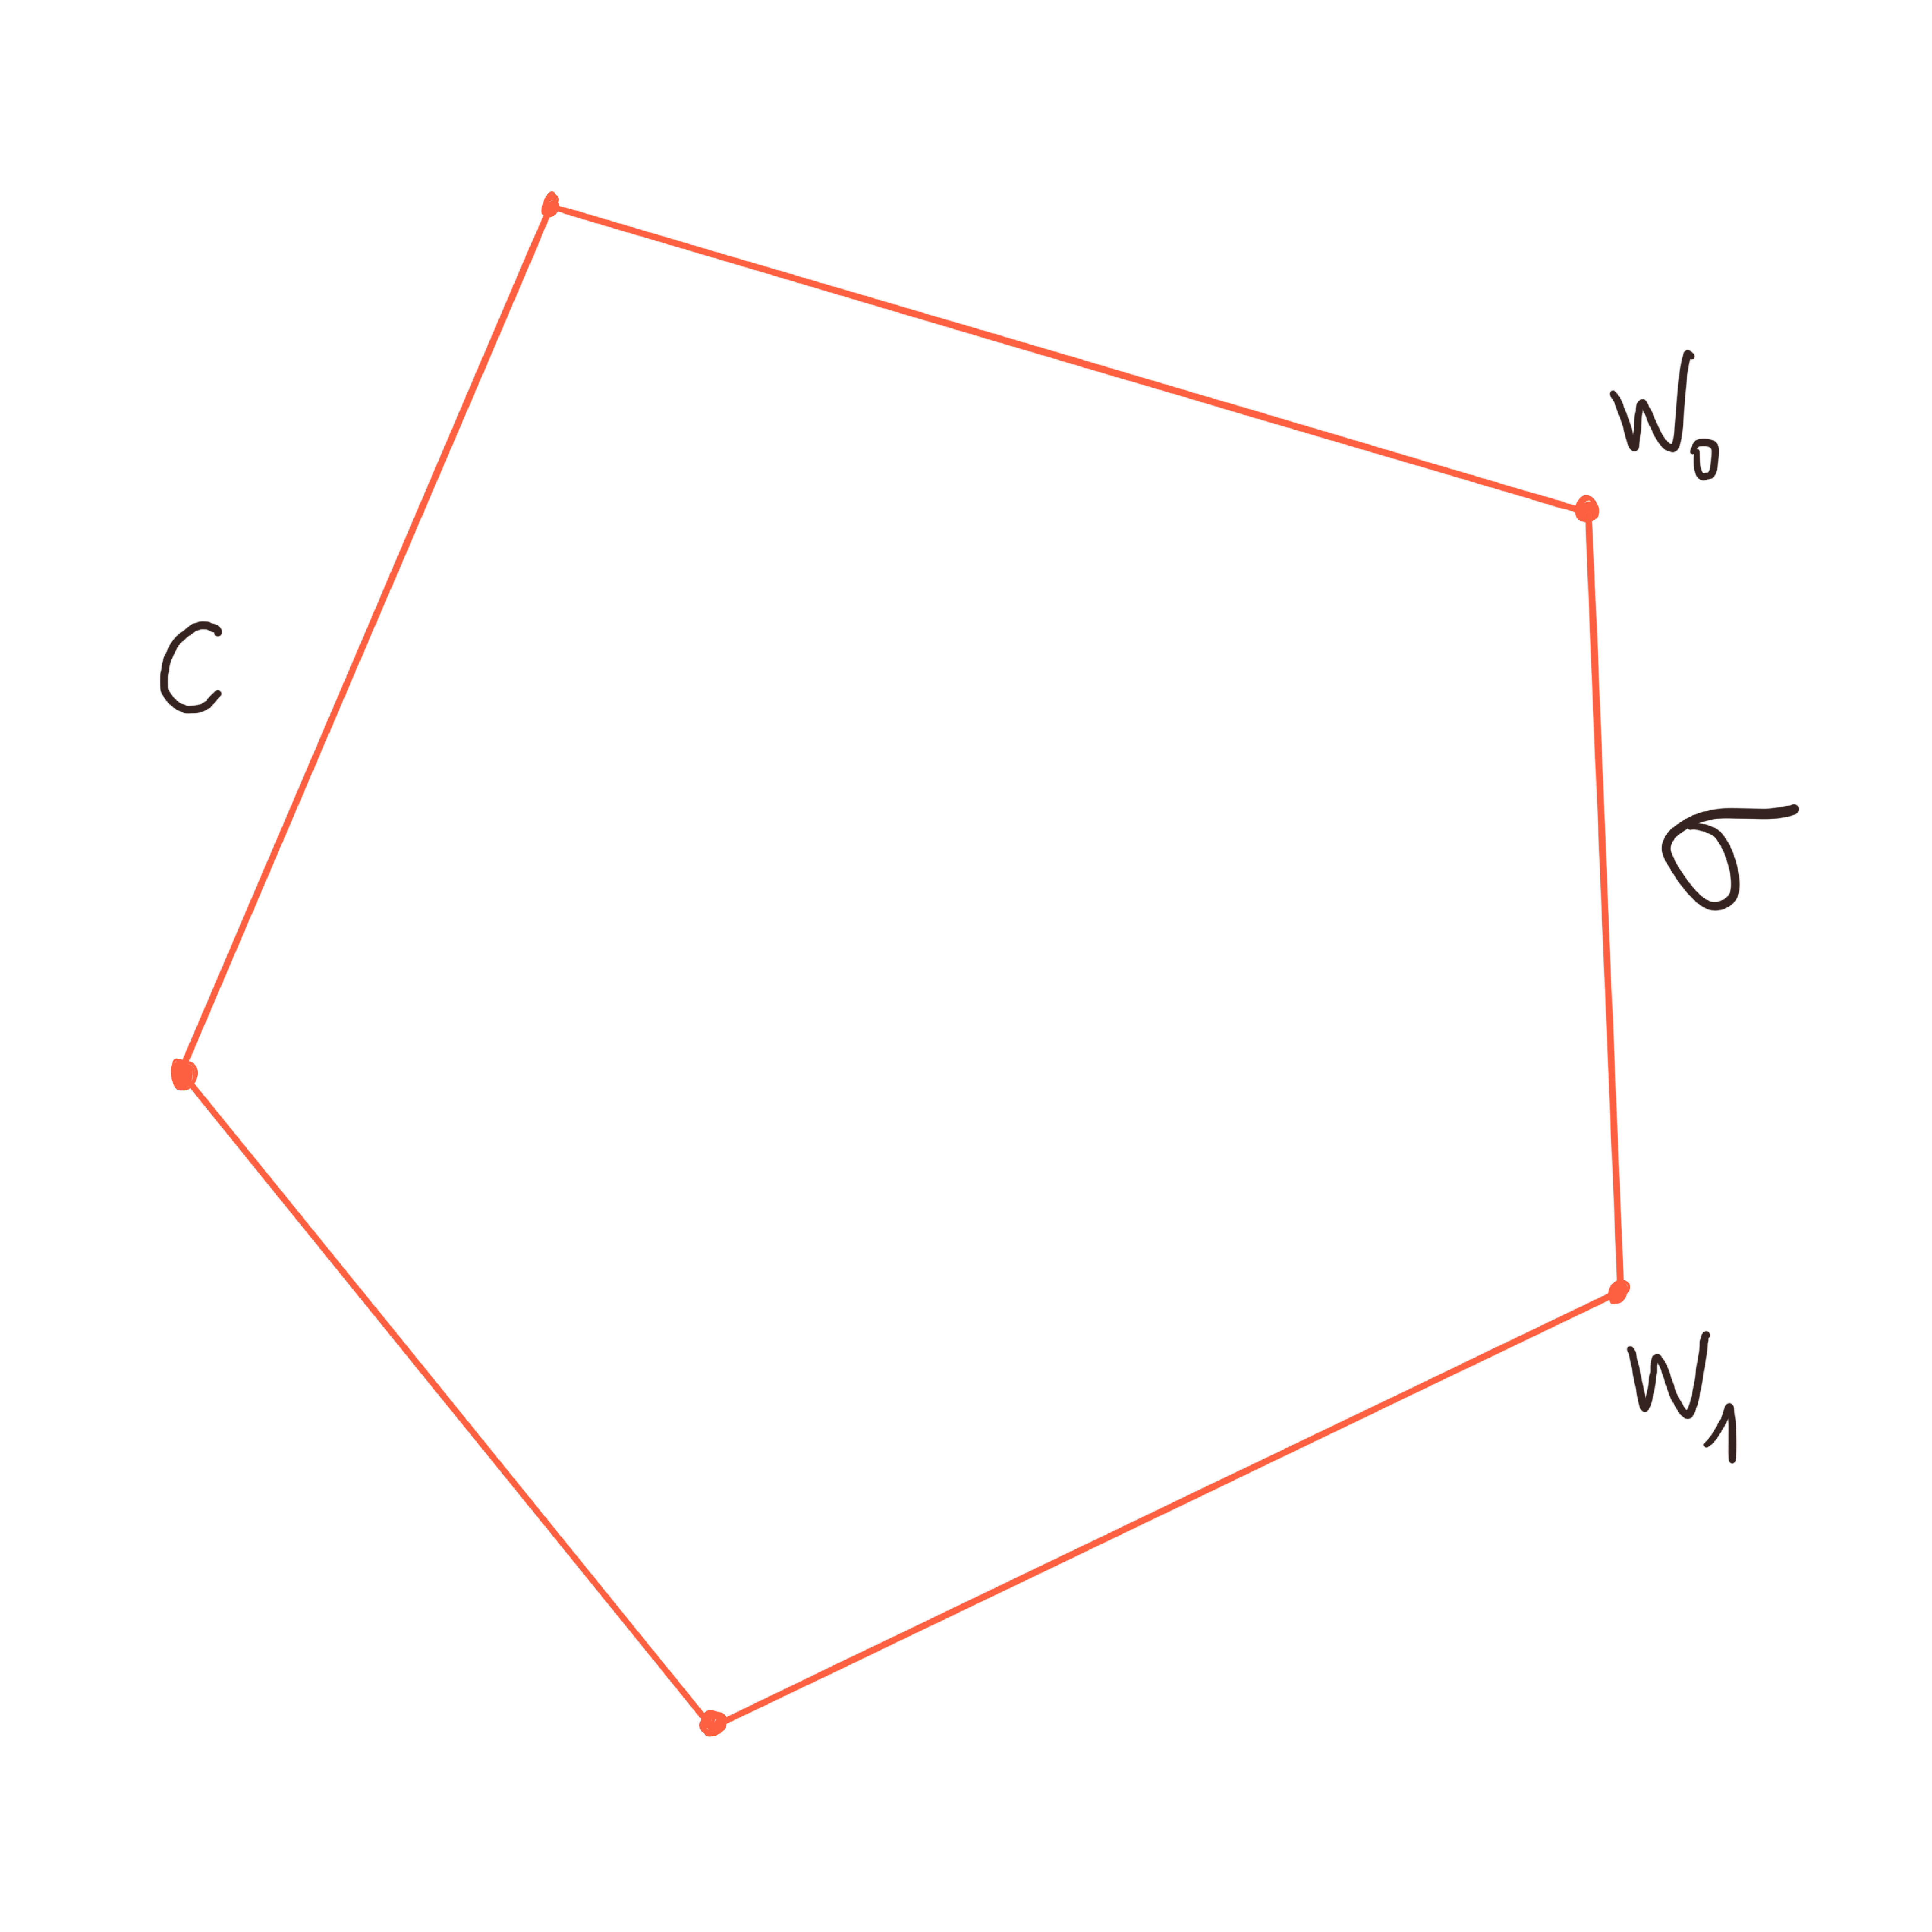
\includegraphics[width = 0.4\textwidth]{beamer/close-2}
\end{frame}

\begin{frame}
	\frametitle{The class \texttt{Homology}}
	\begin{itemize}
		\item If it is not zero, then, before \( \sigma \) appears, its faces formed a cycle
			not homologous to zero. Therefore its homology class was a nontrivial element of the
			corresponding homology group. \pause
		\item Once \( \sigma \) appears, it is covered and so it dies. \pause
	\end{itemize}

	\centering
	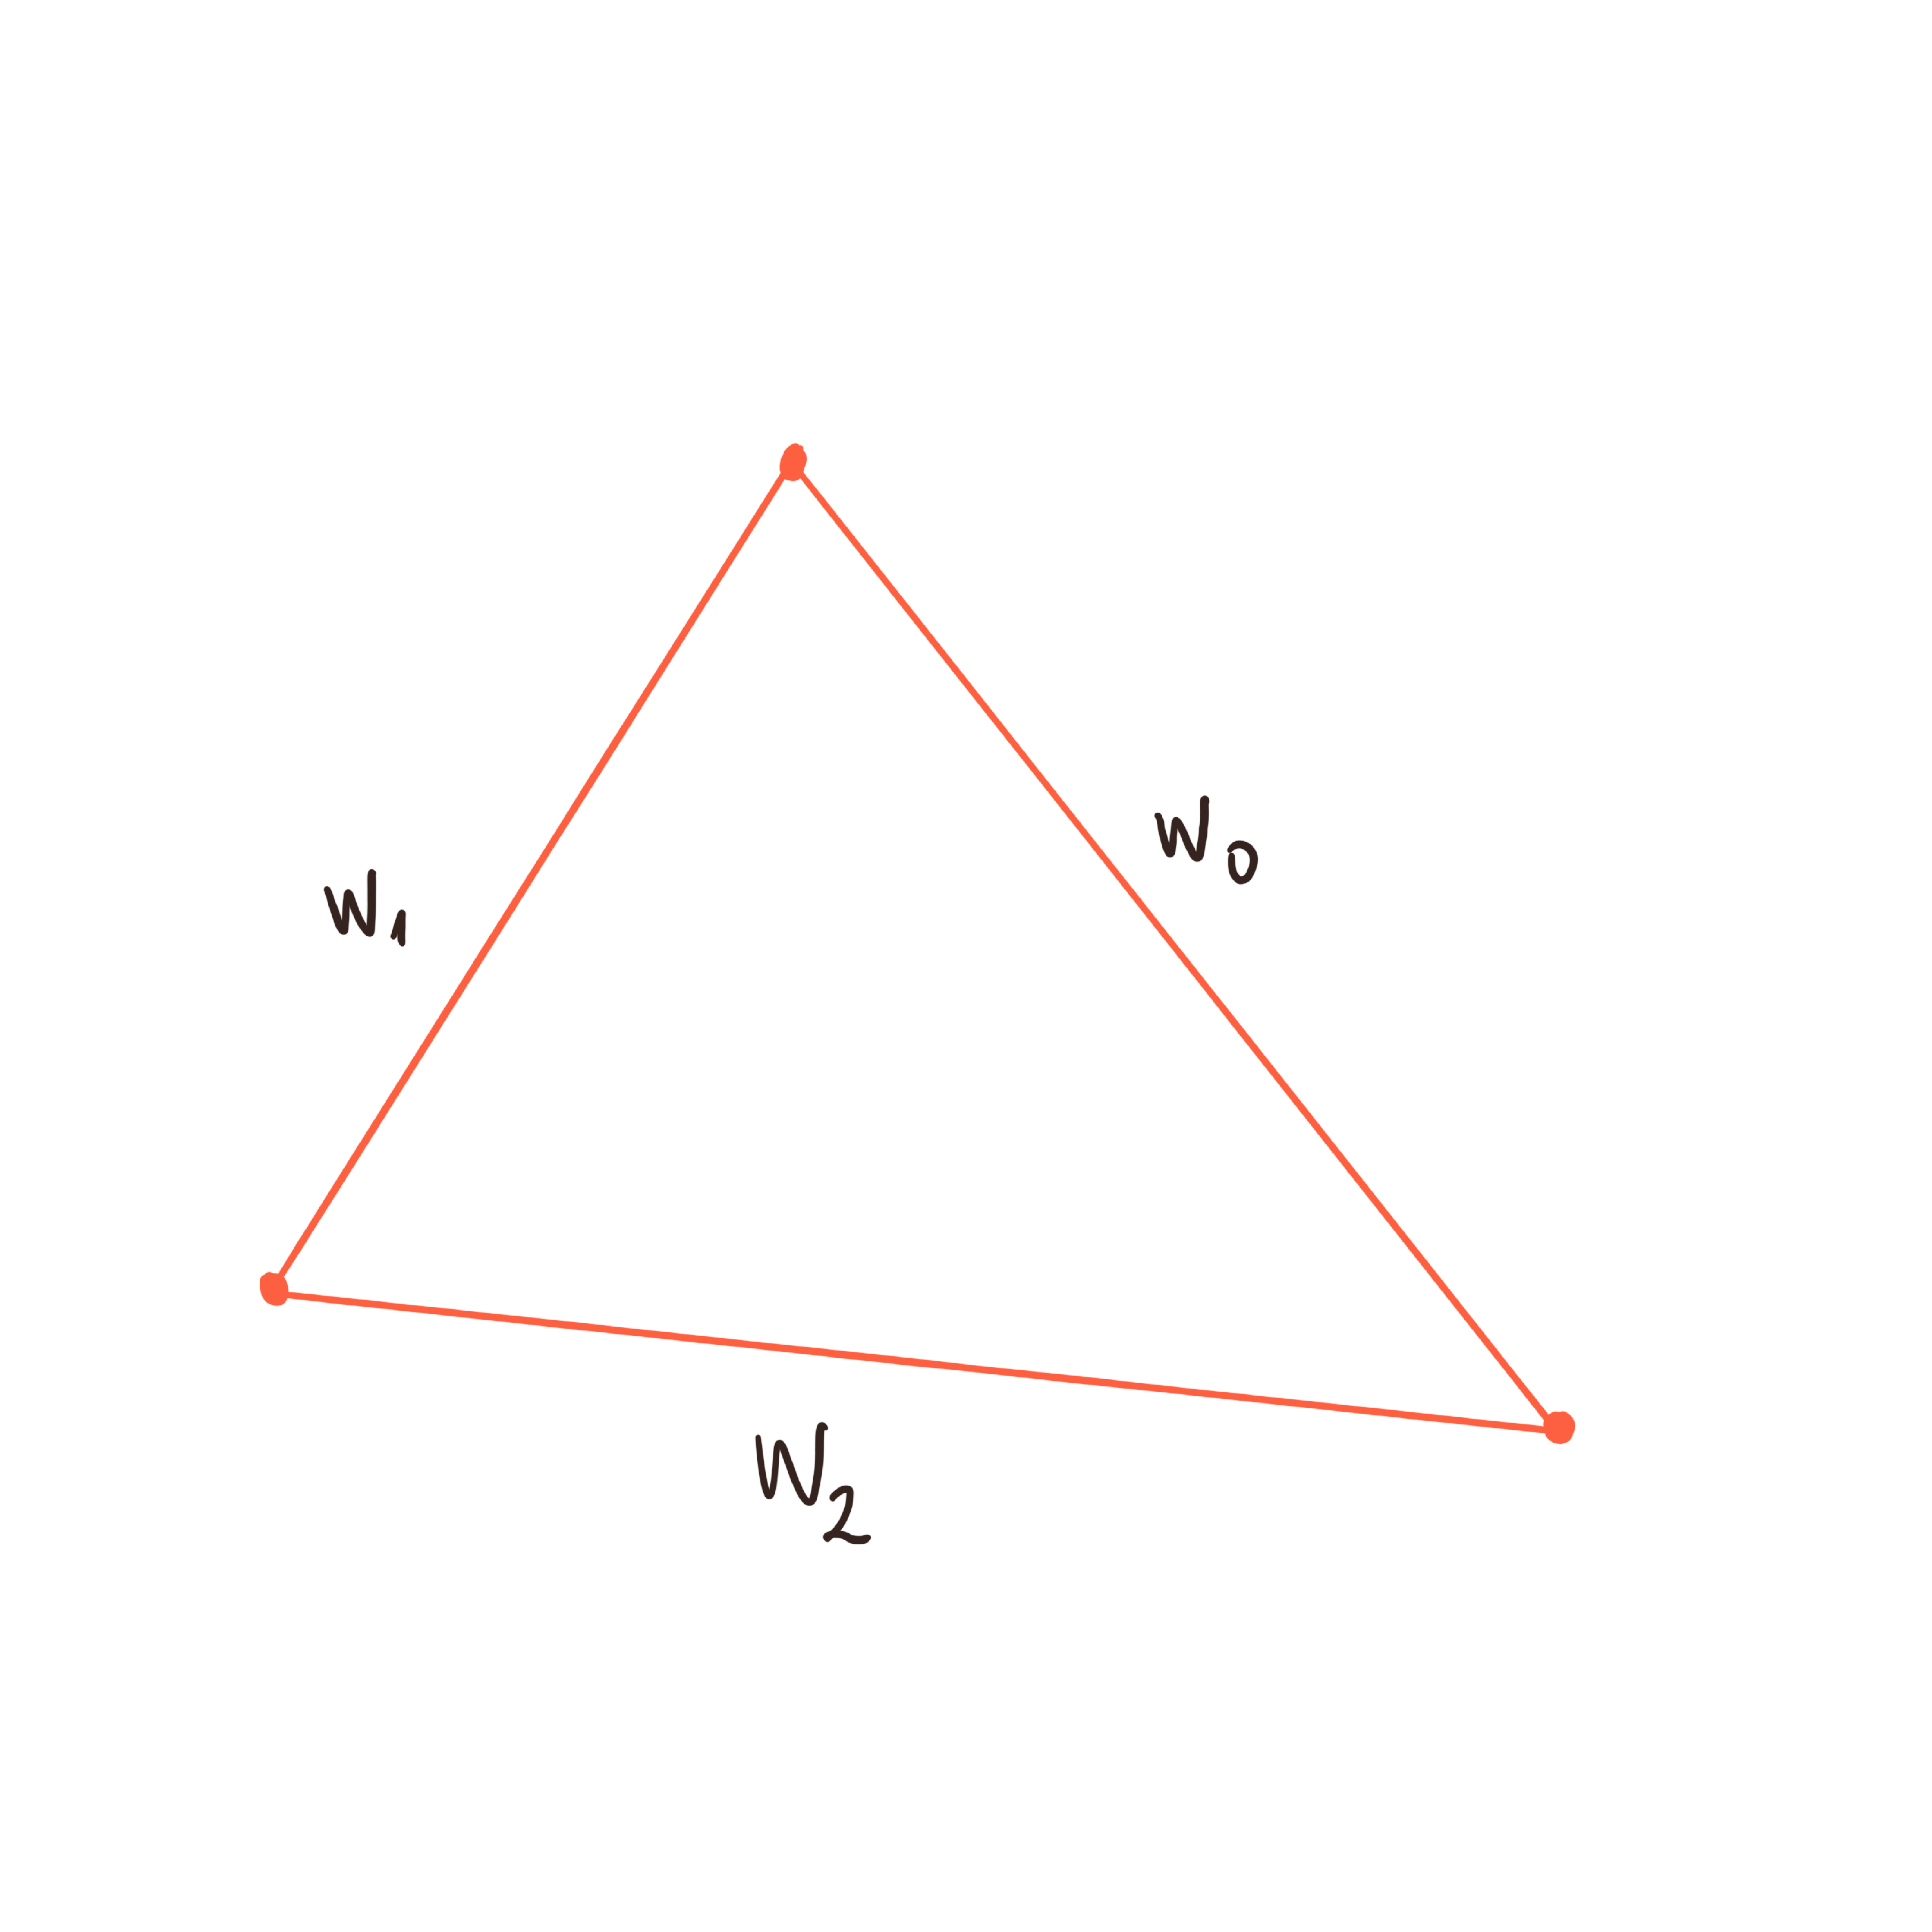
\includegraphics[width = 0.4\textwidth]{beamer/cover-1}
	\hfill
	\pause
	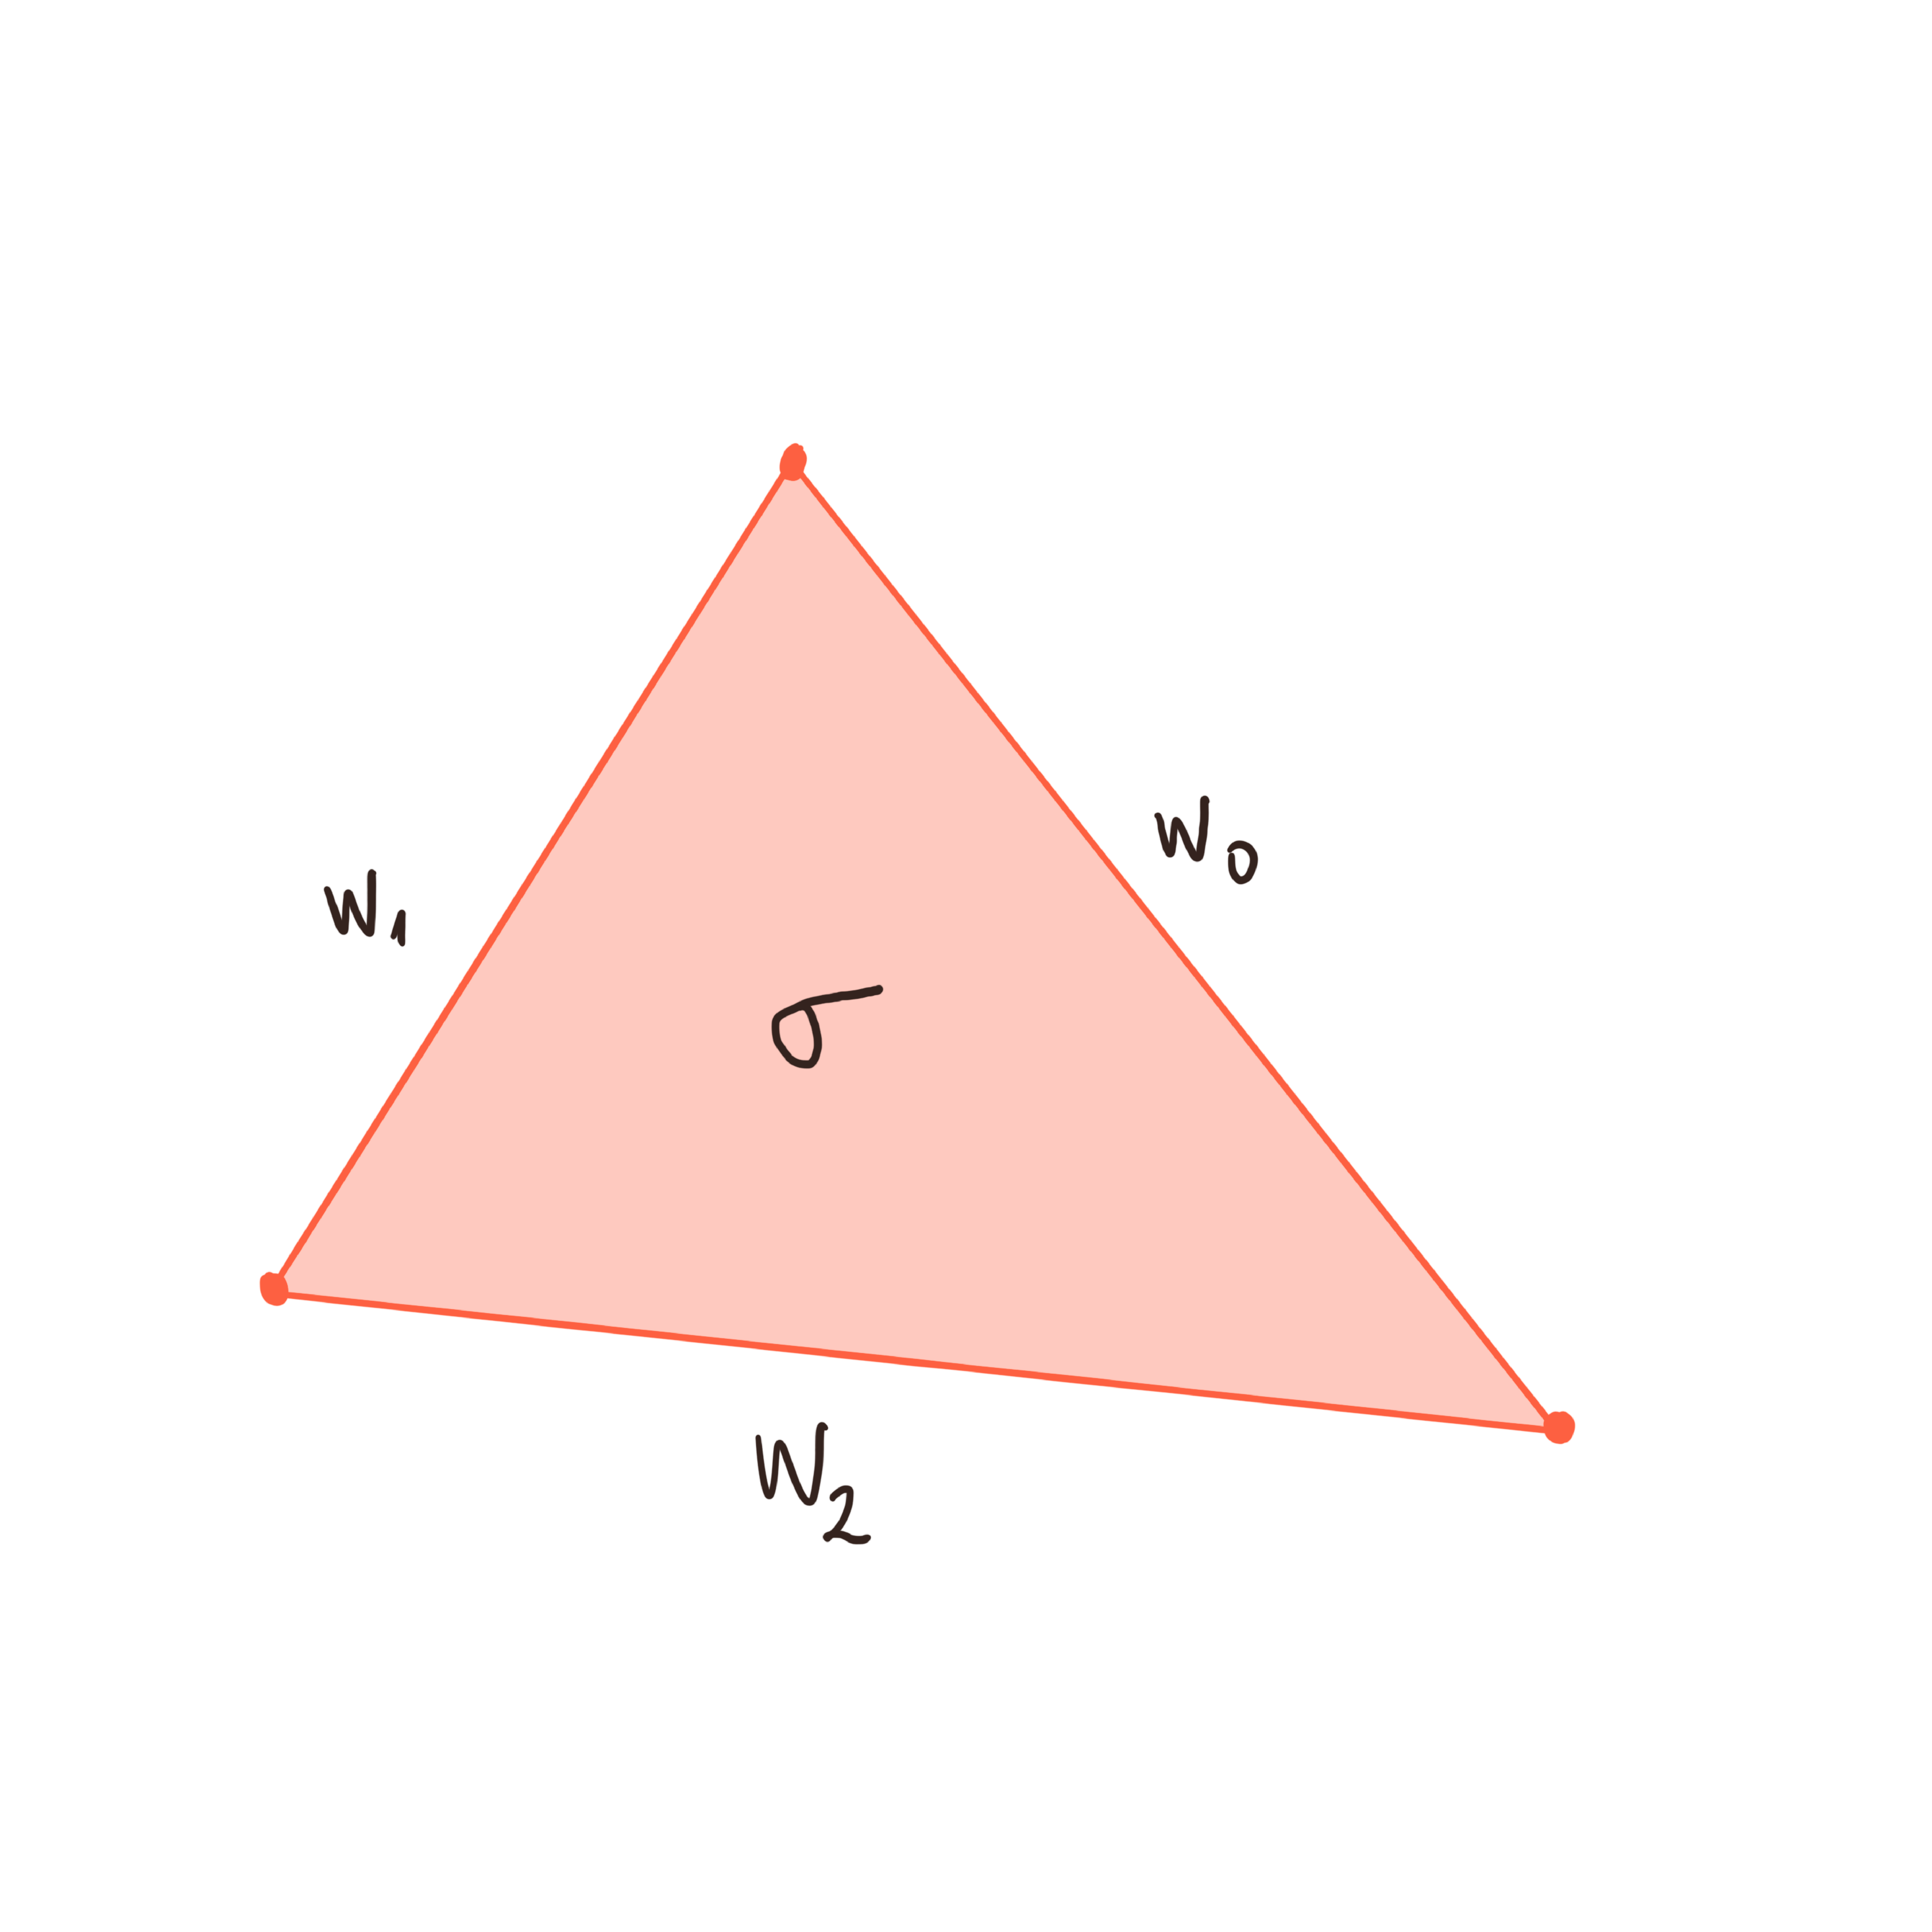
\includegraphics[width = 0.4\textwidth]{beamer/cover-2}
\end{frame}

\begin{frame}
	\frametitle{The persistence data}
	The lifetime and size at death of every class in the zeroth homology group is stored and
	plotted. Outliers will be those classes with few members and long lifetimes, since they
	took a long time to merge into larger clusters. 

	\pause

	Visually, outliers will be those points in the lower right corner of the plot. 
\end{frame}

\section{The results}
\begin{frame}
	\frametitle{A run with toy data}
	\centering
	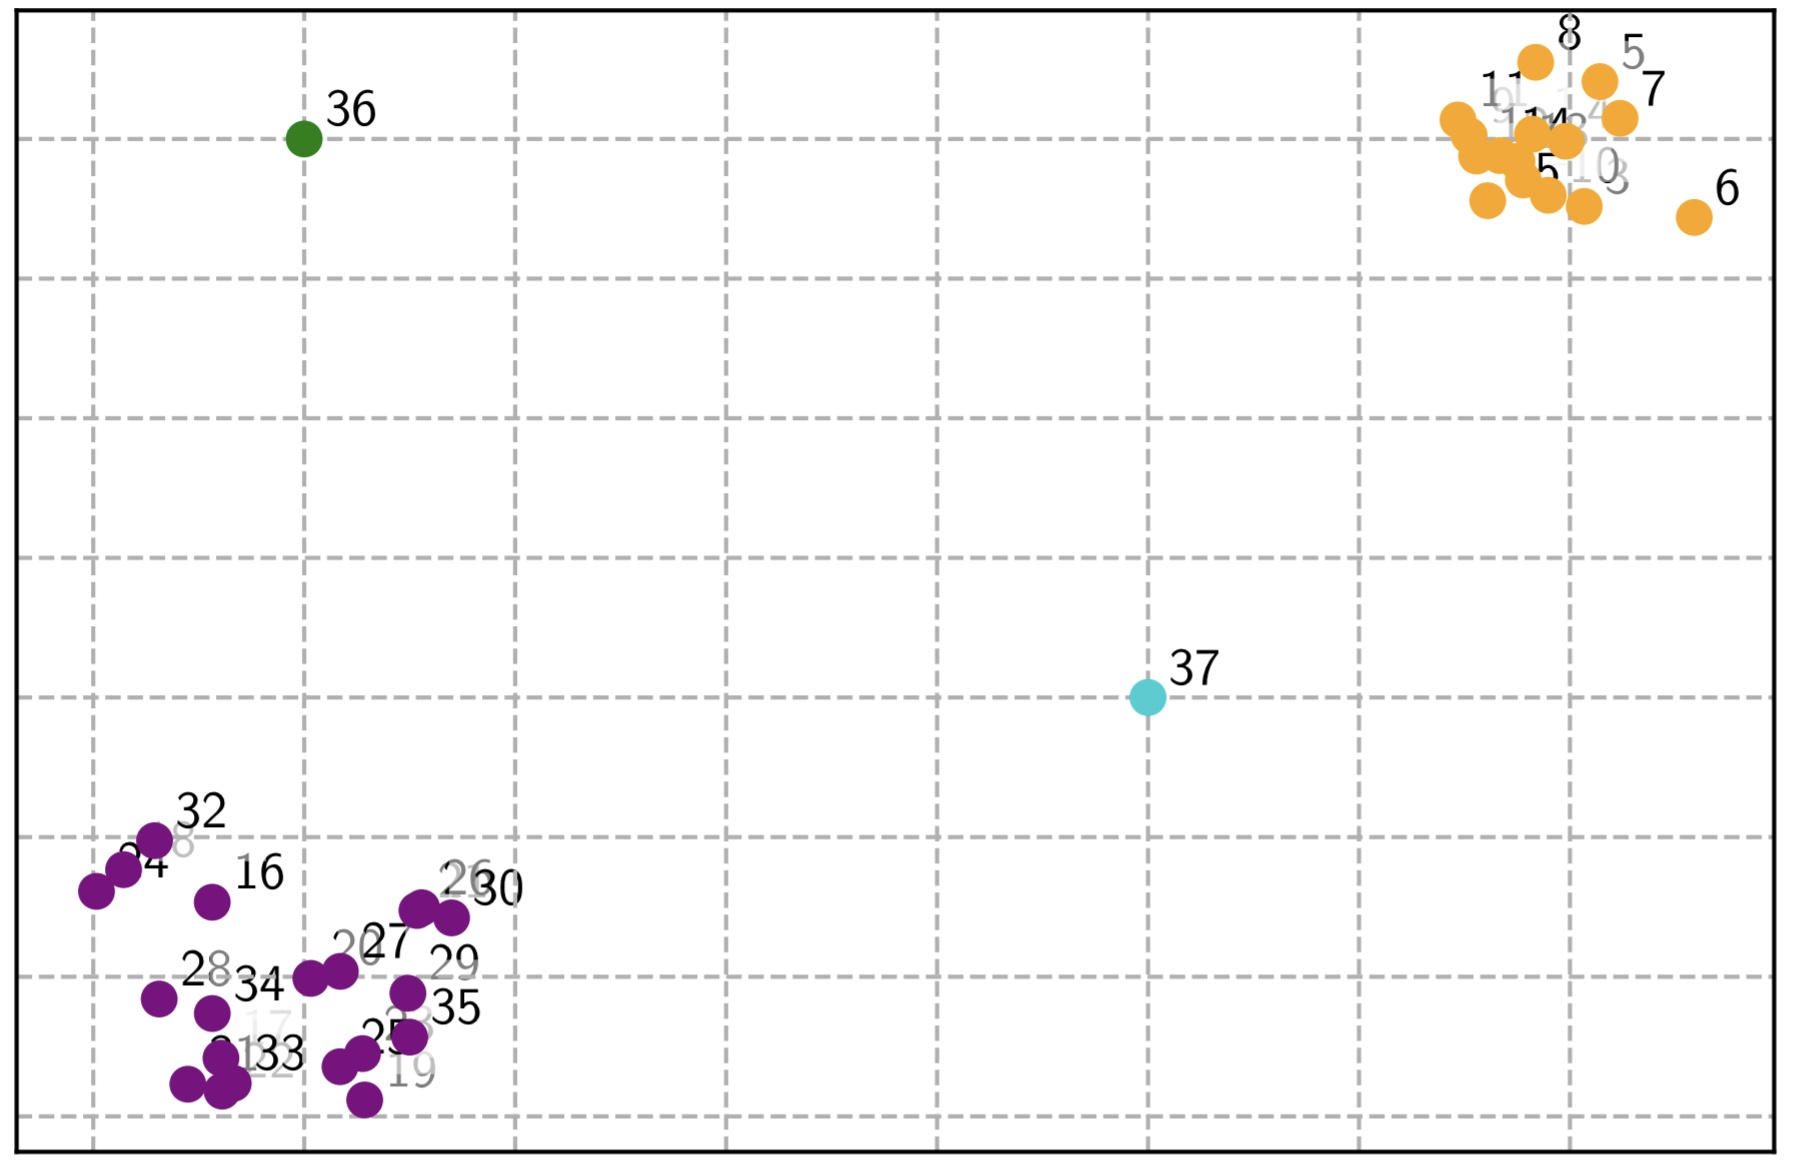
\includegraphics[width=0.9\textwidth]{beamer/clusters}
\end{frame}

\begin{frame}
	\frametitle{A run with toy data}
	\centering
	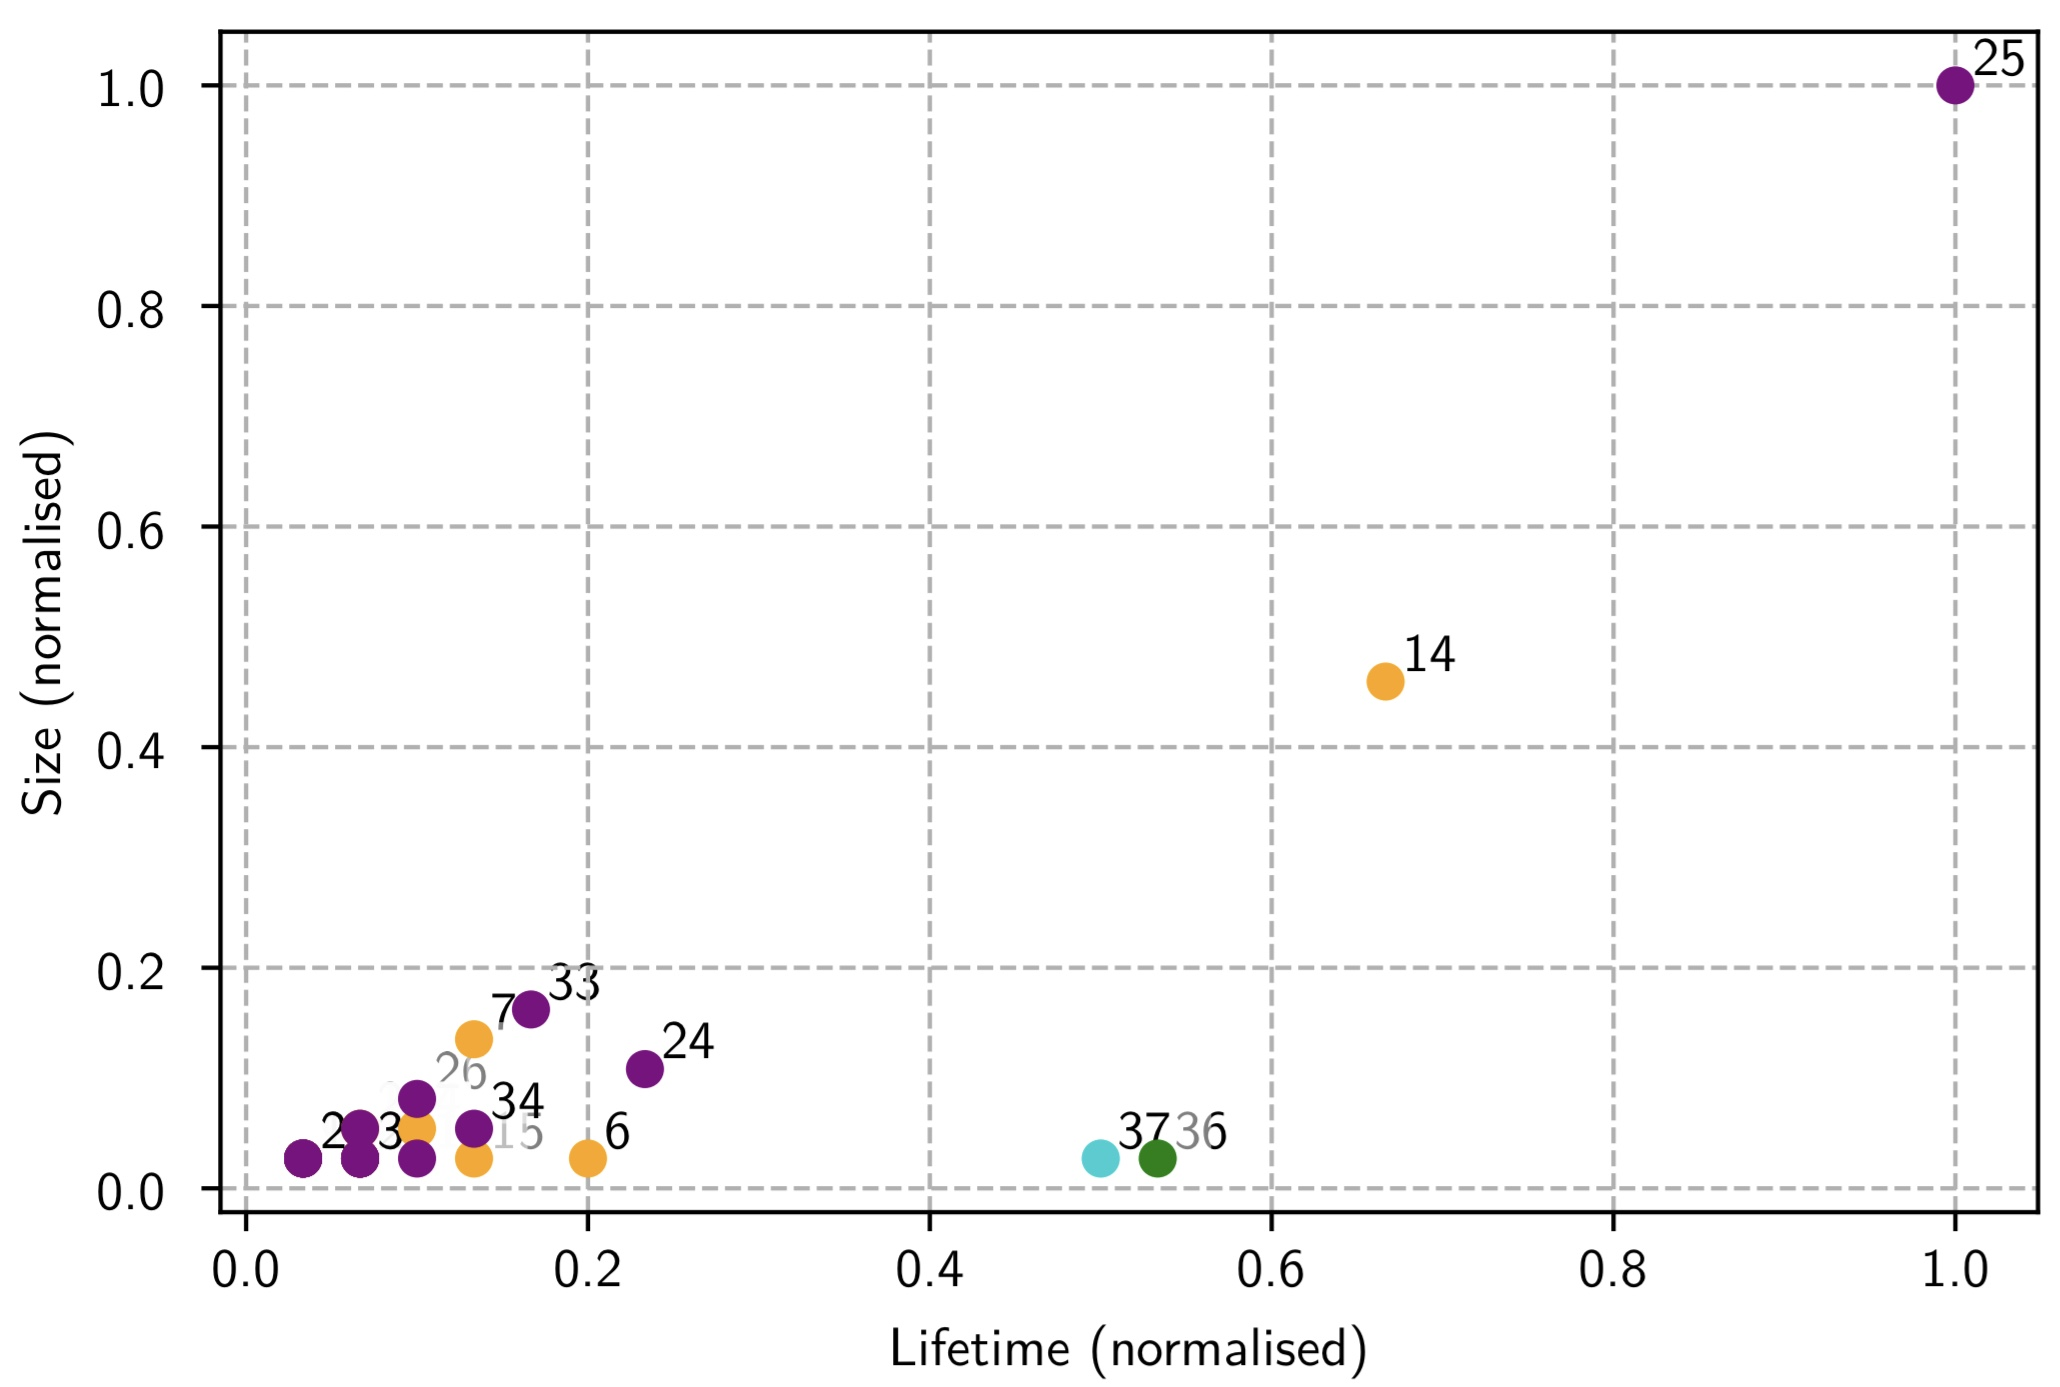
\includegraphics[width=0.9\textwidth]{beamer/toy-results}
\end{frame}

\begin{frame}
	\frametitle{A run with real data}
	\begin{itemize}
		\item The detector was run with a data set consisting of 26 radiomic features measured
			from 20 different patients. These are the result of a previous study carried out at
			VHIO. \pause
		\item There are also genomic features corresponding to the same 20 patients. \pause
		\item The detector was run on both sets to compare the clustering structure. 
	\end{itemize}
\end{frame}

\begin{frame}
	\frametitle{A run with real data}
	\centering
	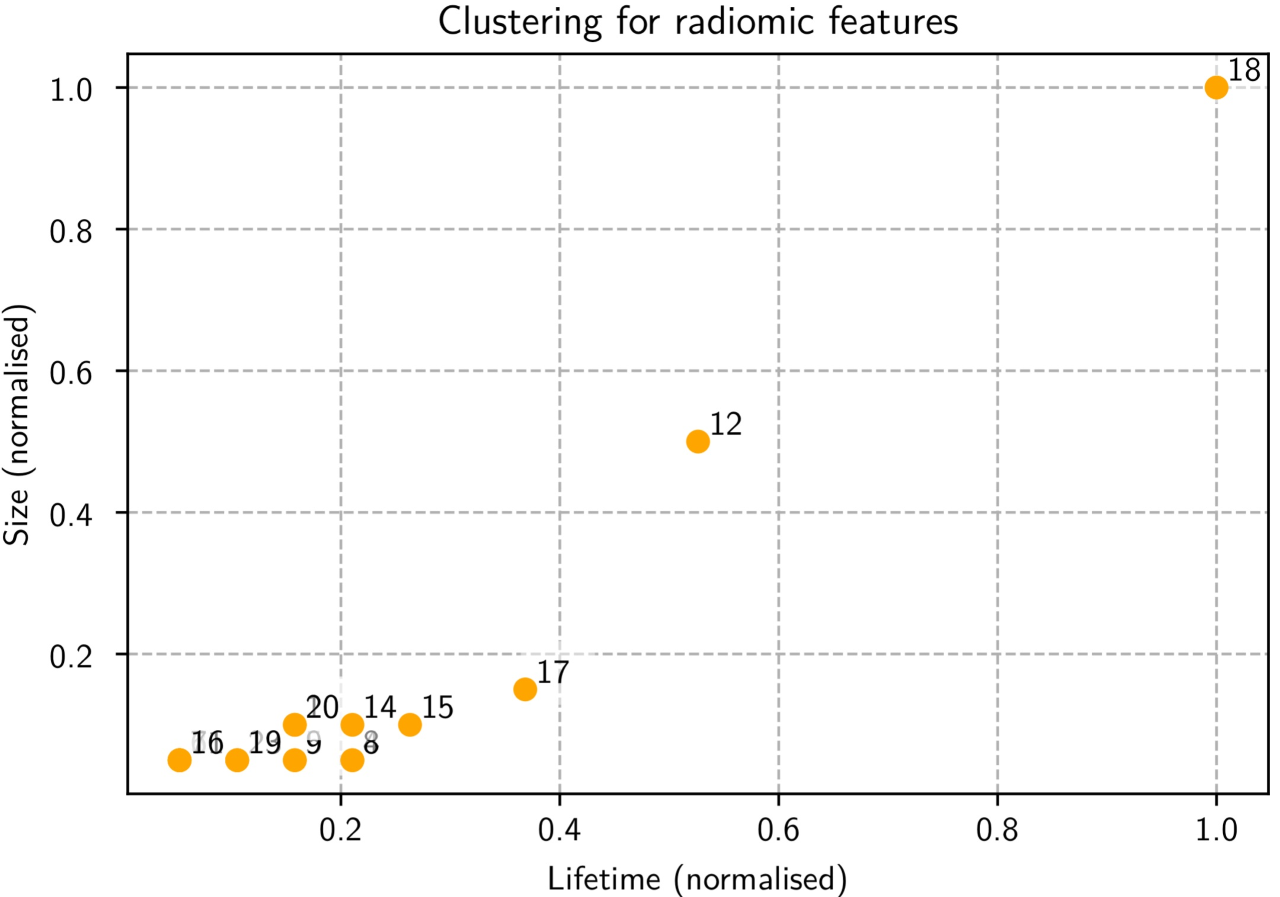
\includegraphics[width = 0.9\textwidth]{beamer/radiomic}
\end{frame}

\begin{frame}
	\frametitle{A run with real data}
	\centering
	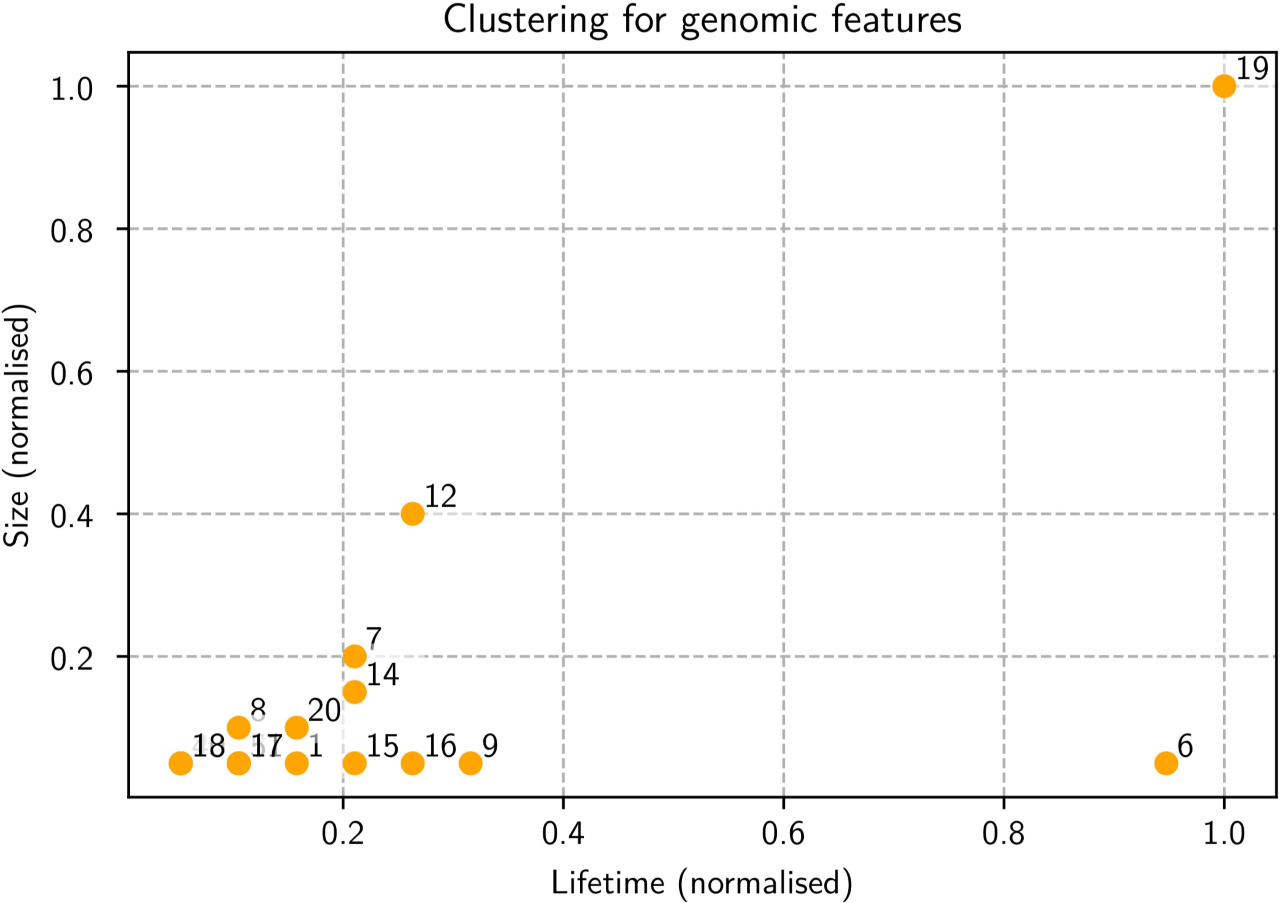
\includegraphics[width = 0.9\textwidth]{beamer/genomic}
\end{frame}

\begin{frame}
	\frametitle{Conclusions}
	\begin{itemize}
		\item Detector appears to properly detect outliers, and gives a quantitative measure
			of ``outlierness''. \pause
		\item The results from the real dataset are awaiting an assesment from VHIO on their
			medical significance. \pause
		\item Further considerations: efficiency, edgecase testing, higher dimensional
			homology. 
	\end{itemize}
\end{frame}
\end{document}
